\documentclass[12pt]{extarticle}
\usepackage{geometry}
\geometry{
a4paper,
total={170mm,257mm},
left=20mm,
top=20mm,
headheight=12pt
}
\usepackage[parfill]{parskip} % Activate to begin paragraphs with an empty line rather than an indent
\usepackage{graphicx} % Use pdf, png, jpg, or eps§ with pdflatex; use eps in DVI mode
% TeX will automatically convert eps --> pdf in pdflatex
		
\usepackage{amssymb,amsmath,amsthm}
\usepackage{commath}
\usepackage{longtable}
\usepackage[hyphens]{url}
\usepackage[dvipsnames]{xcolor}
\usepackage[unicode=true,colorlinks=true,urlcolor=CadetBlue,citecolor=black,linkcolor=black]{hyperref}
\usepackage{booktabs}
\usepackage{pgfplotstable} % http://mirrors.ctan.org/graphics/pgf/contrib/pgfplots/doc/pgfplotstable.pdf
\PassOptionsToPackage{hyphens}{url} % url is loaded by hyperref
\usepackage{authblk}
\usepackage{subcaption}
\captionsetup[subfigure]{labelformat=empty}
\usepackage[font=small,labelfont=bf]{caption}
\usepackage{longtable}
\usepackage{gensymb,siunitx}
\usepackage{cleveref}

%SetFonts
% newtxtext+newtxmath
\usepackage{newtxtext} %loads helv for ss, txtt for tt
\usepackage{amsmath}
\usepackage[bigdelims]{newtxmath}
\usepackage[T1]{fontenc}
\usepackage{textcomp}
%SetFonts

\renewcommand{\baselinestretch}{1.5}

% less space before sections 
% \@startsection {NAME}{LEVEL}{INDENT}{BEFORESKIP}{AFTERSKIP}{STYLE} 
%            optional * [ALTHEADING]{HEADING} 
\makeatletter
 \renewcommand\section{\@startsection {section}{1}{\z@}%
     {-2.5ex \@plus -1ex \@minus -.2ex}%
     {1.3ex \@plus.2ex}%
    {\Large\bfseries}}
    
% Species names
%% Meta-Command for defining new species macros
\usepackage{xspace}

\newcommand{\species}[3]{%
  \newcommand{#1}{\gdef#1{\textit{#3}\xspace}\textit{#2}\xspace}}
  
\species{\yeast}{Saccharomyces cerevisiae}{S.~cerevisiae}
\species{\calbicans}{Candida albicans}{C.~albicans}
\species{\cneoformans}{Cryptococcus neoformans}{C.~neoformans}

% Yoav & Lee commands
\newcommand*{\tr}{^\intercal}
\let\vec\mathbf
\newcommand{\matrx}[1]{{\left[ \stackrel{}{#1}\right]}}
\newcommand{\diag}[1]{\mbox{diag}\matrx{#1}}
\newcommand{\goesto}{\rightarrow}
\newcommand{\dspfrac}[2]{\frac{\displaystyle #1}{\displaystyle #2} }
\newtheorem{theorem}{Theorem}
\newtheorem{corollary}{Corollary}
\newtheorem{lemma}{Lemma}
\newtheorem{remark}{Remark}
\newtheorem{result}{Result}
\renewcommand\qedsymbol{} % no square at end of proof
\newcommand{\cl}{\mathbf{L}}
\newcommand{\cj}{\mathbf{J}}
\newcommand{\ci}{I}
\newcommand{\likelihood}{\mathcal{L}}

% line numbers
 \usepackage[displaymath, mathlines]{lineno}
 \renewcommand\linenumberfont{\normalfont\small\sffamily}
\linenumbers
\modulolinenumbers[2]

% genotype commands
\newcommand{\euwt}{\emph{2n}}
\newcommand{\anwt}{\emph{2n+1}}
\newcommand{\eumt}{\emph{2n*}}
\newcommand{\eumtM}{\emph{$2n^*_M$}}
\newcommand{\eumtA}{\emph{$2n^*_A$}}
\newcommand{\anmt}{\emph{2n+1*}}

% Supplementary
\newcommand{\beginsupplement}{%
      	\setcounter{table}{0}
        \renewcommand{\thetable}{S\arabic{table}}%
        \setcounter{figure}{0}
        \renewcommand{\thefigure}{S\arabic{figure}}%
}

% NatBib
\usepackage[super,comma]{natbib}
%\usepackage[round,colon,authoryear]{natbib}

% Title page
% Chromosomal duplication is a transient evolutionary solution to stress
\title{Chromosomal duplication can be an evolutionary detour on the path to adaptation}

% Authors
\renewcommand\Affilfont{\small}

\author[1,2,*]{Ilia Kohanovski}
\author[1,*]{Martin Pontz}
\author[3]{Avihu H. Yona}
\author[1,$\dagger$]{Yoav Ram}

\affil[1]{School of Zoology, Faculty of Life Sciences, Tel Aviv University, Tel Aviv, Israel}
\affil[2]{School of Computer Science, Reichman University, Herzliya, Israel}
\affil[3]{Institute of Biochemistry, Food Science and Nutrition,
Robert H. Smith Faculty of Agriculture, Food and Environment,
The Hebrew University of Jerusalem, Israel}
\affil[*]{These authors contributed equally to this work}
\affil[$\dagger$]{Corresponding author: yoav@yoavram.com}

% Document
\begin{document}
\maketitle

Classifications. Biological Sciences: Evolution, Genetics, Microbiology, Population Biology.

Keywords: aneuploidy, evolutionary model, adaptive evolution

\pagebreak

% Abstract 250 words
\begin{abstract} 
Aneuploidy is common in eukaryotes, often leading to decreased growth and fitness. However, evidence from yeast and fungi, as well as human tumour cells, suggests that specific aneuploidies can be beneficial under stressful conditions and facilitate  adaptation.
In a prominent example, an evolutionary experiment with yeast, populations evolving under heat stress had become aneuploid (chromosome III), only to later revert back to euploid after genetic mutations have accumulated. It has therefore been suggested that aneuploidy serves as a "stepping stone" on the path to adaptation.

Here, we test this hypothesis. First, we apply DNA sequencing to show that mutant alleles common in aneuploid cells are uncommon in the evolved euploid population. 
Second, we develop an evolutionary model with both aneuploidy and  mutation, and fit it to the results of the experiment using a Bayesian inference framework.
We then predict the genotype frequency dynamics during the experiment, demonstrating that the majority of the evolved euploid population likely did not descend from aneuploid cells, but rather directly from the euploid wild-type population.
Our model further predicts that if the experiment was repeated with smaller populations, then a larger fraction of the evolved population would descend from aneuploid cells. 

Together, our results suggest that aneuploidy can be an evolutionary "detour" rather than a "stepping stone": it can delay, rather than facilitate, the adaptation of the population, and cells that become aneuploid may leave less descendants compared to cells that remain diploid.
\end{abstract}

% TODO Significance statement 120 words

\pagebreak 

% Introduction
\section*{Introduction}

%\paragraph{Aneuploidy is common in eukaryotes.}
Aneuploidy is an imbalance in the number of chromosomes in the cell: an incorrect karyotype.
Evidence suggests aneuploidy is very common in eukaryotes, e.g. animals~\citep{Santaguida2015review, Naylor2016, Bakhoum2017}, and fungi~\citep{Pavelka2010, Zhu2016, Robbins2017, Todd2017}.
Aneuploidy has been implicated in cancer formation, progression, and resistance~\citep{Boveri2008, Schvartzman2010, Santaguida2015review, Ippolito2021b}.
It is also common in protozoan pathogens of the Leishmania genus, a major global health concern~\citep{Mannaert2012}, and contributes to the emergence of drug resistance~\citep{Selmecki2009} and virulence~\citep{Moller2018} in fungal pathogens, which are under-studied~\citep{Rodrigues2018}, despite infecting a billion people per year, causing significant morbidity in >150 million and death in >1.5 million people per year~\citep{Selmecki2009, Rodrigues2018}.

%\paragraph{Aneuploidy is generally deleterious.}
Experiments with human and mouse embryos found that most aneuploidies are lethal.
It is also associated with developmental defects and lethality in other multicellular organisms~\citep{Sheltzer2011}. For example, aneuploid mouse embryonic cells grow slower than euploid cells~\citep{Williams2008}.
Similarly, in unicellular eukaryotes growing in benign conditions, aneuploidy usually leads to slower growth and decreased overall fitness~\citep{Niwa2006, Torres2007, Pavelka2010, Sheltzer2011, Kasuga2016, Yang2021}, in part due to proteotoxic stress caused by increased expression in aneuploid cells~\citep{Pavelka2010, Santaguida2015, Zhu2018} and hypo-osmotic-like stress~\citep{Tsai2019}.

%\paragraph{Aneuploidy can lead to adaptation.}
However, aneuploidy can be beneficial under stressful conditions due to the wide range of phenotypes it can produce, some of which are advantageous~\citep{Pavelka2010, Yang2021}.
Thus, aneuploidy can lead to rapid adaptation in unicellular eukaryotes~\citep{Gerstein2015,Torres2010, Hong2014, Rancati2008}, as well as to rapid growth of somatic tumour cells~\citep{Schvartzman2010, Sheltzer2017}.
For example, aneuploidy in \yeast facilitates adaptation to a variety of stressful conditions like heat and pH~\citep{Yona2012}, copper~\citep{Covo2014, Gerstein2015}, salt~\citep{Dhar2011}, and nutrient limitation~\citep{Dunham2002, Gresham2008, Avecilla2022}, with similar results in \calbicans~\citep{Yang2021}.
Importantly, aneuploidy can also lead to drug resistance in pathogenic fungi such as \calbicans~\citep{Selmecki2008, Selmecki2010, Gerstein2018} and \cneoformans~\citep{Sionov2010}, which cause candidiasis and meningoencephalitis, respectively.

%\paragraph{Transient adaptive solution.} 
\citet{Yona2012} demonstrated experimentally the importance of aneuploidy in adaptive evolution. They evolved populations of \yeast under strong heat stress.
The populations adapted to the heat stress within 450 generations, and this adaptation was determined to be due a duplication of chromosome III.
Later on, after more than 1,500 generations, the populations reverted back to an euploid state, while remaining adapted to the heat stress. 
Aneuploidy was therefore suggested to be a \emph{transient adaptive solution}, because it can rapidly appear and fixate in the population under stressful conditions, and can then be rapidly lost when the cost of aneuploidy outweighs its benefit---after the stress is removed, or after "refined" beneficial mutations appear and fixate~\citep{Yona2012}.
Furthermore, it has been suggested that aneuploidy is an evolutionary "stepping stone" that facilitates future adaptation by genetic mutations, which require more time to evolve~\citep{Yona2012,Yona2015}.

%\paragraph{The present study.}
Here, we test the hypothesis that aneuploidy is a an \emph{evolutionary stepping stone} that facilitates adaptive evolution by genetic mutations.
First, we analyze previously unpublished sequencing data from the original experimental populations \citep{Yona2012} to assess if the evolved euploid population is descended from the aneuploid population.
Second, we develop an evolutionary genetic model and fit it to the experimental results of \citet{Yona2012} in order to predict the genotype frequency dynamics in the experimental populations, thereby estimating the frequency of evolved euploid cells that descended from aneuploid cells. 
Our results show that aneuploidy reached high frequencies in the experimental populations, but nevertheless, the majority of cells in the evolved euploid populations likely did not descend from aneuploid cells, but rather directly from wild-type euploid cells.
These results suggest that aneuploidy can be an evolutionary detour, rather than a stepping stone, on the path to adaptation.


%%%%%%%%%%%%%%%%%%%%%%%%%%%
% Results
\section*{Results}
In the heat-stress experiment of \citet{Yona2012}, four populations of \yeast evolved under \SI{39}{\celsius}.
Aneuploidy fixed in all four experimental repetitions in the first 450 generations.
Two of the repetitions, marked $H2$ and $H4$, carried no large-scale duplications other than a chromosome III trisomy.
These two repetitions continued to evolve under the same conditions, wherein aneuploidy was eliminated by generation 1,700 and 2,350 in $H4$ and $H2$, respectively.

\paragraph{Empirical frequencies of mutant alleles.} 
For each of two evolved populations ($H2$ and $H4$) we sequenced the ancestral population (generation 0), the aneuploid population (generation 450), and the evolved euploid population (generation 1,700 or 2,350) to estimate the mutant allele frequencies (\Cref{table:mutations_H2,table:mutations_H4}). 
Overall, between 100 and 173 mutant alleles were detected with at least a single read in the six populations that were sampled. 
Disregarding 45 and 40 alleles that were present in the ancestral populations at a frequency >10\%, the aneuploid and euploid populations carried a large number of mutant alleles: 82 and 95, respectively, in repetition $H2$, and 60 and 66 in repetition $H4$.

Surprisingly, out of all these mutant alleles, none was present at a frequency >20\% in both the aneuploid and the evolved euploid populations. 
Furthermore, a high mutant allele frequency in the aneuploid population implies a low frequency in the evolved euploid population, and vice-versa (Spearman's correlation coefficient $\rho=-0.64$ and $-0.66$ in the two experimental repetitions; \Cref{fig:mutation_frequencies}), such that mutant alleles frequent in the aneuploid populations decreased in frequency when aneuploidy was lost.
Moreover, for the 18 mutant alleles with high frequency in the aneuploid populations (>20\%), the highest frequencies in the euploid populations were 15.4\%, 16\%, 16.3\% and 19.6\% (the rest were below 15\%).
Similarly, for the 48 mutant alleles with high frequency in the evolved euploid populations, the highest frequencies in the aneuploid populations were 2.7\%, 7.7\%, and 11.1\% (the rest were below 1\%). 
These results suggest evolved euploid cells are unlikely to descend from aneuploid~cells.

%%%%%%%% Fig mutation frequencies
\begin{figure}[h]
  \centering
    \includegraphics[width=\textwidth]{../figures/mutation_frequencies.pdf}      
  \caption{
    \textbf{Frequencies of mutant alleles in the experimental populations are negatively correlated.} 
    Frequencies of mutant alleles when trisomy was widespread in the population (y-axis) and after it was eliminated (x-axis) in two experimental repetitions (circles for $H2$ and triangles for $H4$) from \citet{Yona2012}. Mutant alleles with >20\% in the aneuploid population were <20\% in the euploid population, and vice versa (the upper-right quadrant is empty), suggesting that the majority of evolved euploid cells did not descend from the most common aneuploid genotypes. 
Alleles with frequency below and above 10\% in the ancestral populations are in black and gray, respectively. 
Solid black line is a linear orthogonal distance regression line (slope=$-0.559$, intercept=$0.164$; a regression through alleles that reach at least 20\% in one of the populations has slope=$-0.645$ and intercept=$0.297$).
Dashed vertical and horizontal lines show allele frequencies 20\%. Error bars show standard error of the mean accounting for the number of reads.
}
  \label{fig:mutation_frequencies}
\end{figure}

%%%%%%%%%%%%%%%%%%%%%%%%%%%%%%%%%%

\paragraph{Evolutionary genetic model.} 
To explore the dynamics during the evolutionary experiments, we developed an evolutionary genetic model, fitted the model to empirical data, and used it to predict the genotype frequency dynamics, or specifically, the fraction of the evolved euploid population descended from aneuploid cells. 

The model includes the effects of natural selection, genetic drift, aneuploidy, and mutation, and follows a population of cells characterized by their genotype: 
euploid wild-type, \euwt, is the ancestral diploid genotype; 
euploid mutant, \eumt, has a diploid karyotype and a single beneficial mutation; 
aneuploid wild-type, \anwt, has an extra chromosome due to a chromosome duplication event; and
aneuploid mutant, \anmt, has and extra chromosome and a beneficial mutation.
Fitness values of the different genotypes are denoted by $w_{\euwt}$, $w_{\eumt}$, $w_{\anwt}$, and $w_{\anmt}$, and the rate of mutation and aneuploidy are denoted by $\mu$ and $\delta$. See \Cref{fig:models} for an illustration of the model.

We fitted this model to the experimental results\citep{Yona2012} -- time for fixation (>95\%) and for loss (<5\%) of aneuploidy -- using approximate Bayesian computation with sequential Monte Carol (ABC-SMC)~\citep{Sisson2009}, thereby inferring the model parameters: rates aneuploidy and mutation and the fitness of all genotypes.
We then sampled posterior predictions for the genotype frequency dynamics using the estimated parameter values and compared different versions of the model to test additional hypotheses about the evolutionary process.


%%%%%%%% Fig illustration
\begin{figure}[t]
  \centering
    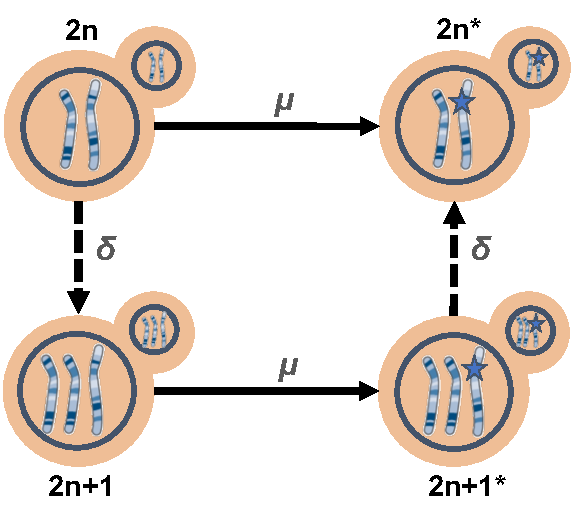
\includegraphics[height=1.8in]{../figures/Fig1-A.pdf}      
  \caption{
    \textbf{Model Illustration.}
    There are four genotypes in our model: euploid wild-type, \euwt; euploid mutant, \eumt; aneuploid wild-type, \anwt; and aneuploid mutant, \anmt.
    Overall there are two possible trajectories from \euwt\; to \eumt.
    Arrows denote transitions between genotypes, with transitions rates $\mu$ for the beneficial mutation rate and $\delta$ for the aneuploidy rate.
   }
  \label{fig:models}
\end{figure}

%%%%%%%%%%%%%%%%%%%%%%%%

\paragraph{Estimated rates and fitness effects of aneuploidy and mutation.} 
We inferred the posterior distribution of model parameters~(\Cref{fig:posterior}). 
We report parameter estimates using the MAP (maximum a posteriori) and providing the 50\% HDI (highest density interval) in square brackets. See Supplementary Material for sensitivity analysis.
%% estimates generated by MAP-and-hdi.ipynb

% without back transitions:
The estimated beneficial mutation rate, $\mu=2.965\cdot10^{-6}\ [2.718\cdot10^{-7}-3.589\cdot10^{-6}]$, corresponds to a mutation target size of $\sim 10^{4}$, assuming the mutation rate per base pair is roughly $2\cdot10^{-10}$ (ref.~\citep{Zhu2014}) or $3.3\cdot10^{-10}$ (ref.~\citep{Lynch2008}).
The estimated aneuploidy rate, $\delta=1.72\cdot10^{-3}\ [1.47\cdot10^{-3}-2.786\cdot10^{-3}]$ is higher than in previous studies: for chromosome III in diploid \yeast, \citet{Zhu2014} estimated $6.7\cdot10^{-6}$ chromosome gain events per generation, and \citet{Kumaran2013} estimate $3.0-4.3\cdot10^{-5}$ chromosome loss events per generation (95\% confidence interval).
The estimated fitness values are $w_{\anwt}=1.022\ [1.021-1.023]$,
$w_{\anmt}=1.025\ [1.024-1.026]$,
$w_{\eumt}=1.028\ [1.026-1.029]$, all relative to the fitness of \euwt, which is set to $w_{\euwt}=1$. 
Thus, we can infer that the cost of chromosome III trisomy is $c = w_{\eumt}-w_{\anmt} = 0.003$ (or 0.3\%) and the benefit of trisomy is $w_{\anwt}-1-c=0.019$ (1.9\%), whereas the benefit of the beneficial mutation is $w_{\eumt}-1=0.028$ (2.8\%).

If we allow for transitions (mutation, chromosome loss and gain) to less-fit genotypes (e.g., \eumt\ to \anmt), then we infer similar but slightly different values, see Supplementary Material.

% FIG posterior
%% generated with posterior-plot.ipynb
\begin{figure}[h]
  \centering
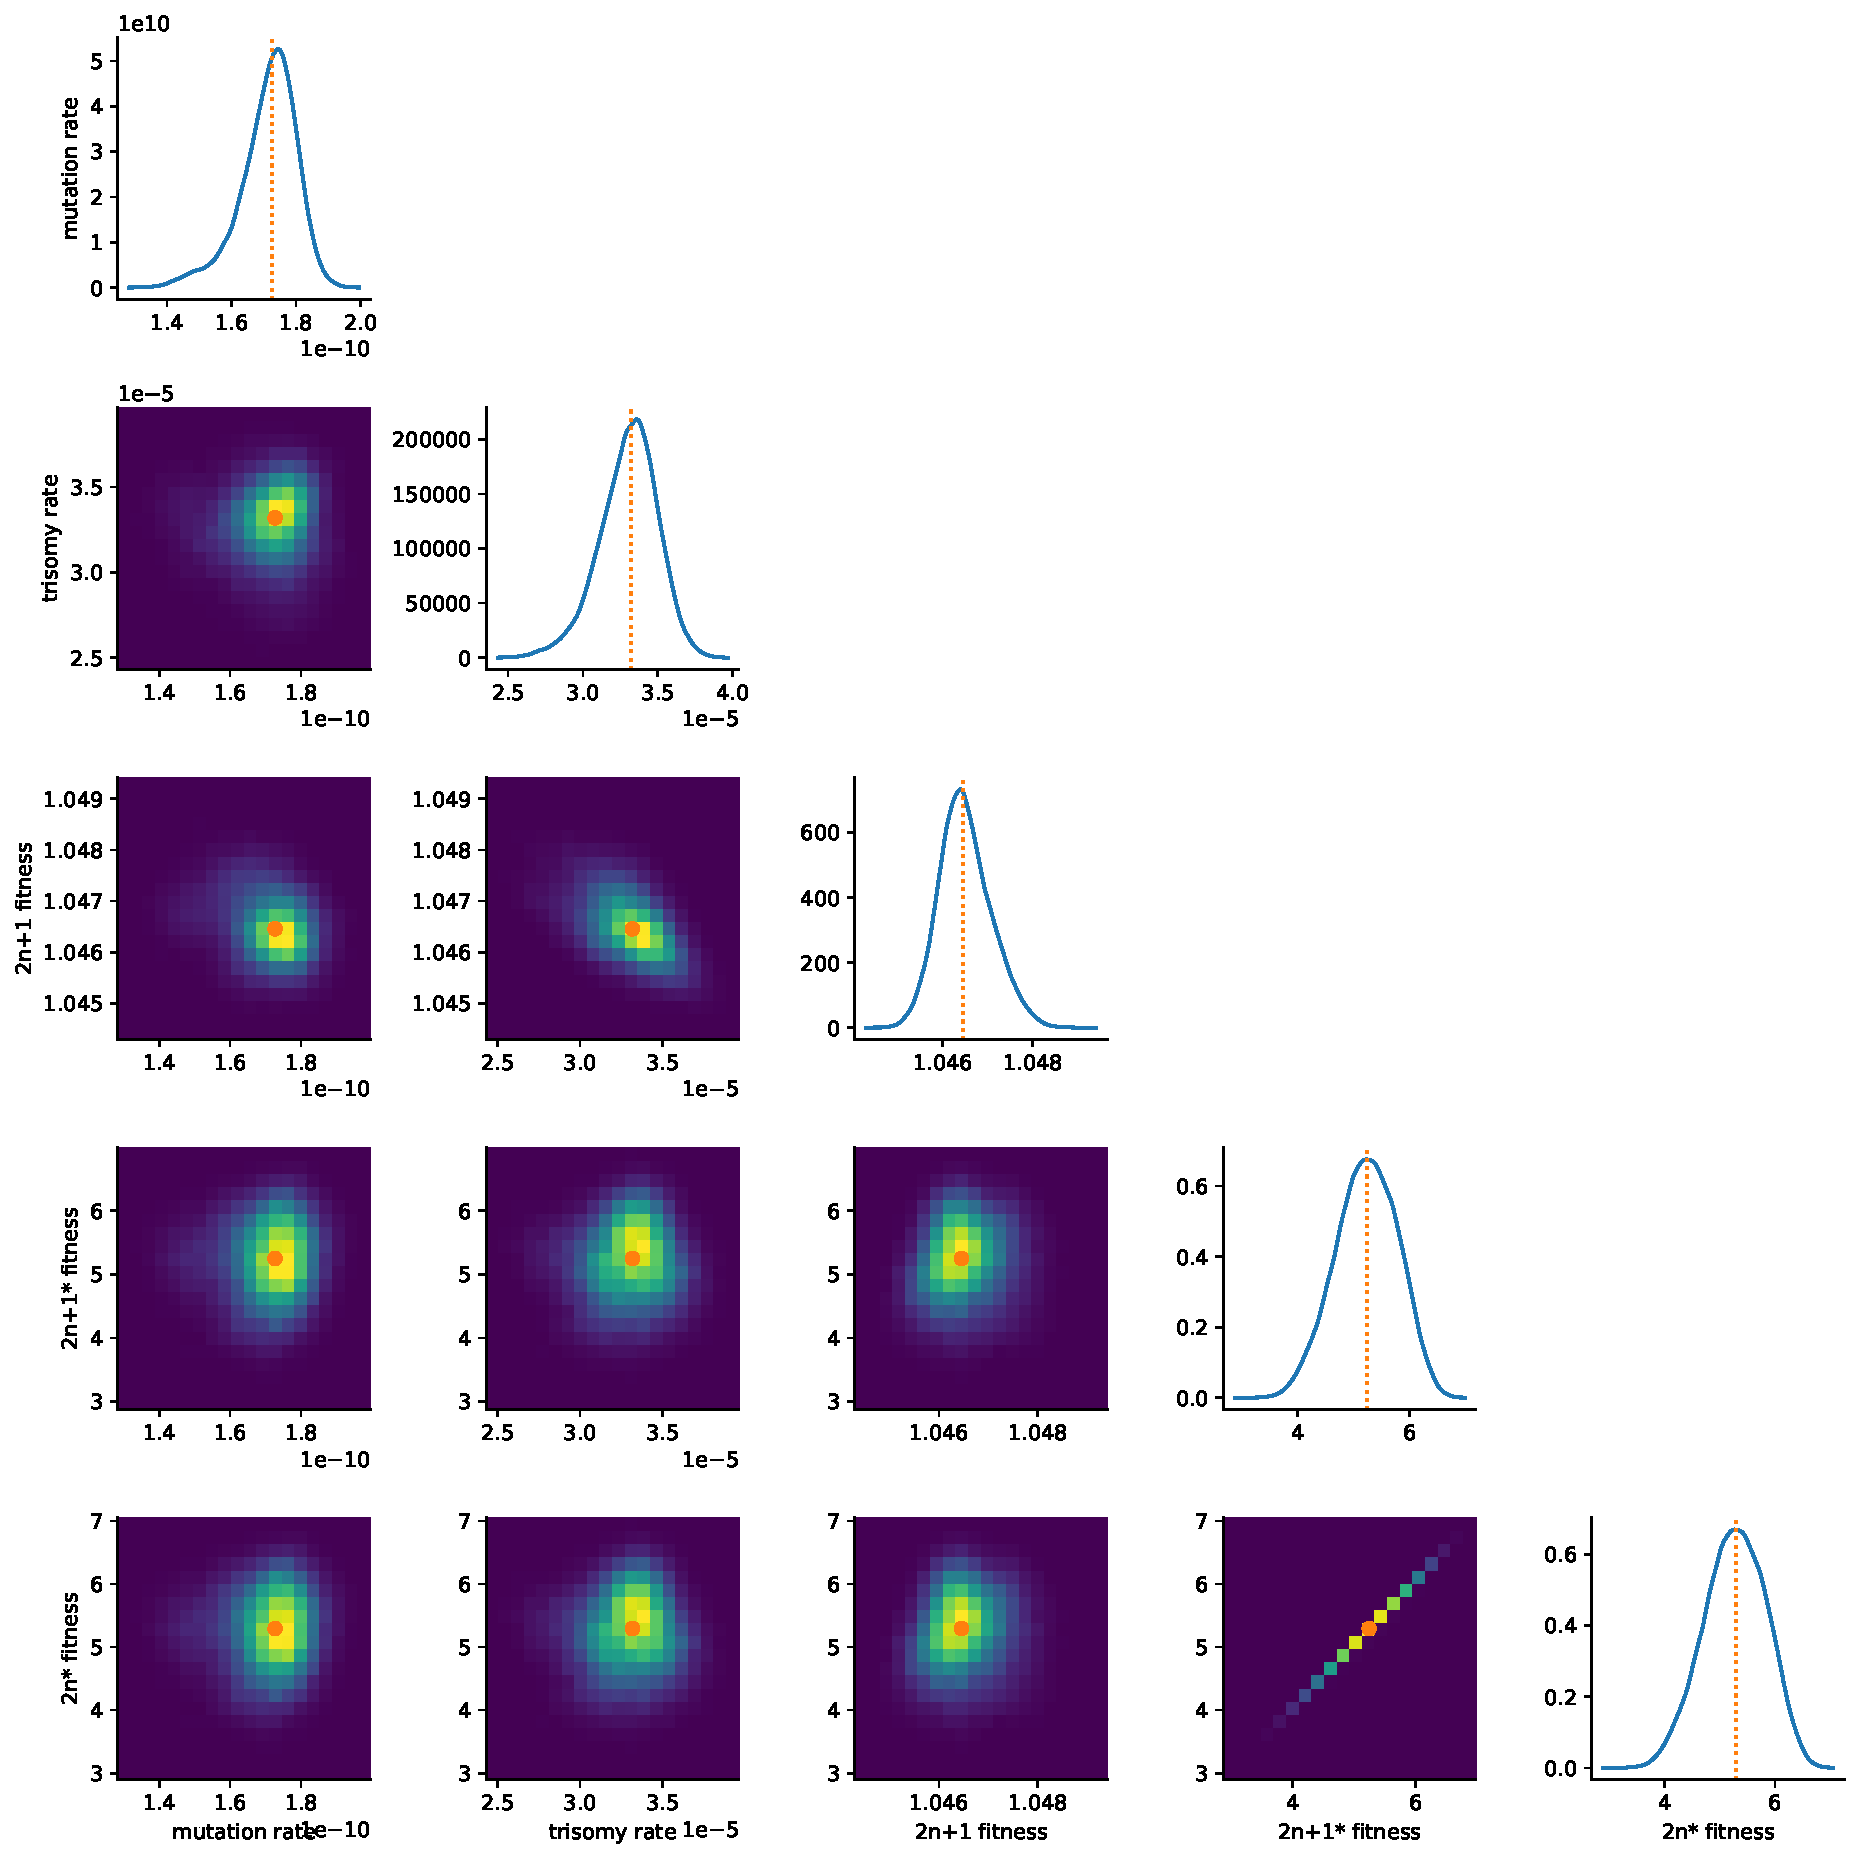
\includegraphics[width=0.8\textwidth]{../figures/posterior.pdf}
  \caption{
  \textbf{Posterior distribution of model parameters.}
On the diagonal, the marginal posterior distribution of each model parameter. 
Below the diagonal, the joint posterior distribution of pairs of model parameters (dark purple and bright yellow for low and high density, respectively). Red markers and orange lines for the joint MAP estimate (which may differ from the marginal MAP, as the marginal distribution integrates over all other parameters).
} 
  \label{fig:posterior}
\end{figure}
%%%%%%%%%%%%%%%%%%%%%%

\paragraph{Model comparison and goodness-of-fit.}

% Fig model comparison 
%% generated with with-aneuploidy_vs_no_aneuploidy.ipynb
\begin{figure}[h!]
  \begin{subfigure}{0.5\textwidth}
      \centering
      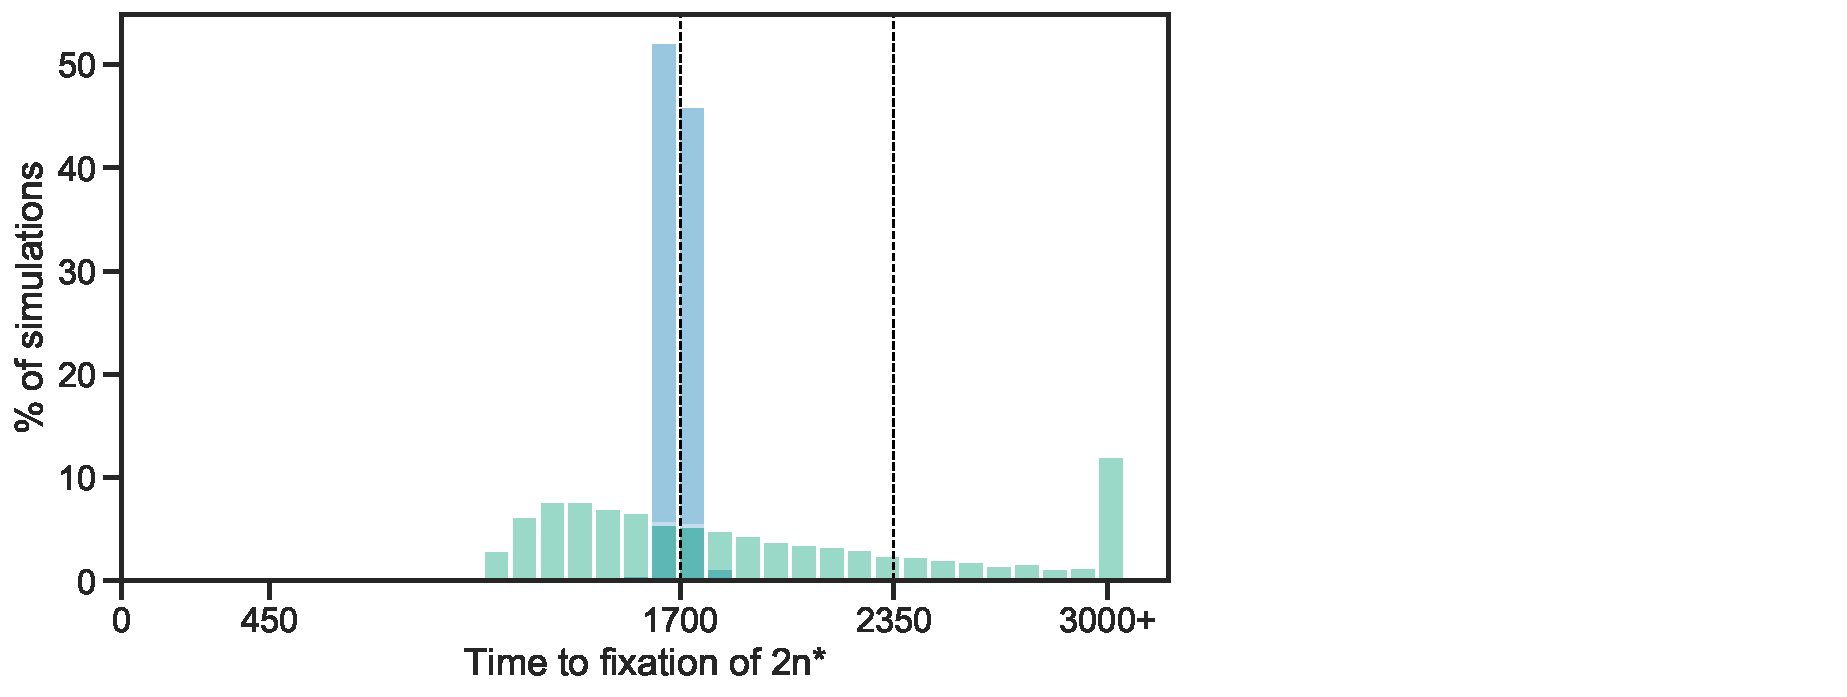
\includegraphics[width=\textwidth]{../figures/fixation-plot-a.pdf}      
      \label{fig:fit}
  \end{subfigure}
  \begin{subfigure}{0.5\textwidth}
      \centering
      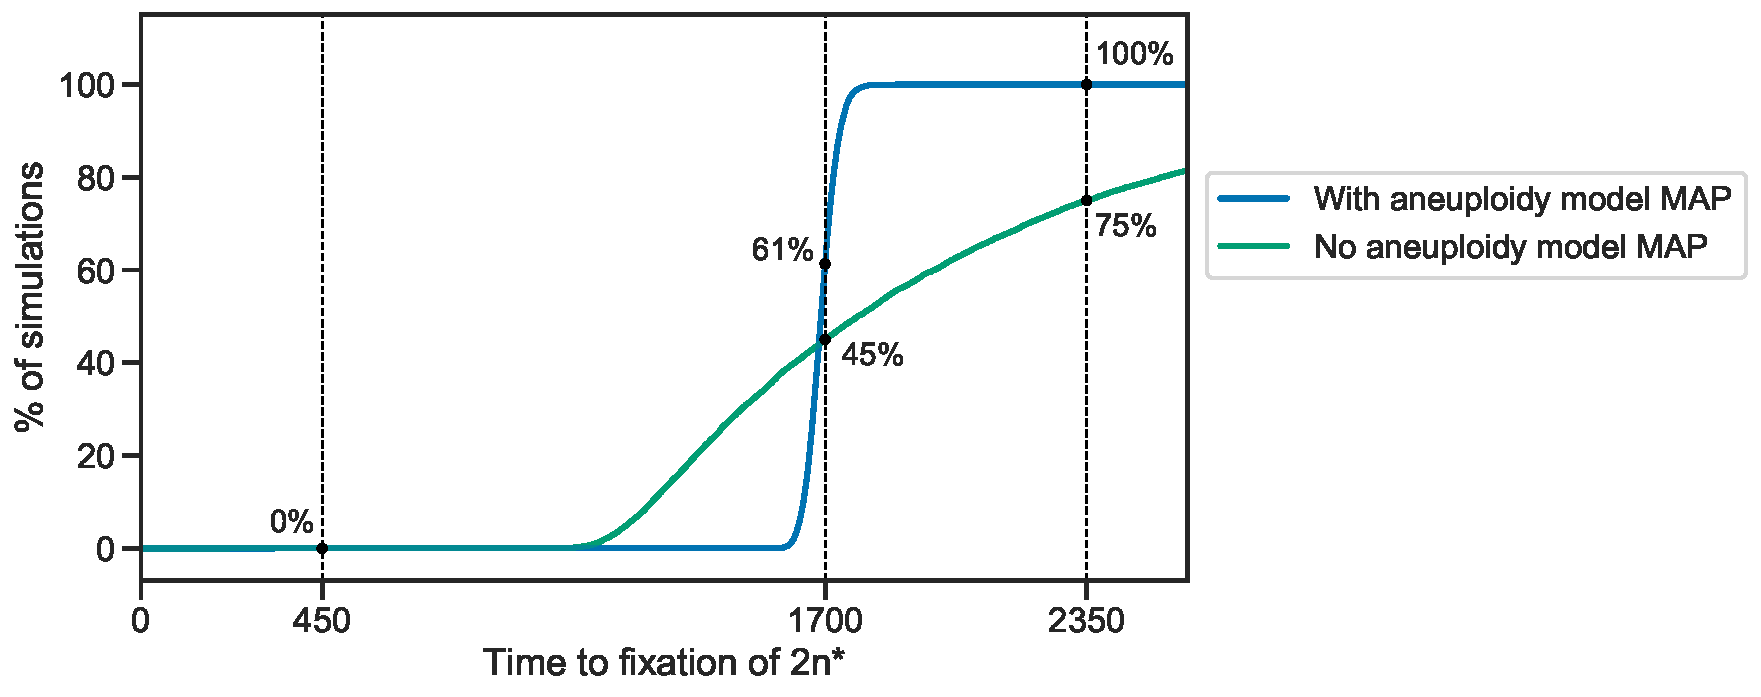
\includegraphics[width=\textwidth]{../figures/fixation-plot-b.pdf}      
      \label{fig:fit-cumulative}
  \end{subfigure}
  \caption{
    \textbf{Model fit with and without aneuploidy.}
    The distribution of time to fixation of \eumt\ (i.e., adaptation time) in $10,000$ simulations using MAP parameters of the model with beneficial aneuploidy (blue; $\delta>0, \; w_{\euwt}<w_{\anwt}<w_{\anmt}<w_{\eumt}$) compared to alternative models: a model with the same parameter values but without aneuploidy (gray, $\delta=0$, concentrated at $t=450$); a model fitted to the data assuming no aneuploidy (green, $\delta=0$); a model fitted to the data assuming neutral aneuploidy (yellow, $\delta>0, \; w_{\anwt}=w_{\euwt}, \; w_{\anmt}=w_{\eumt}$); and a model with beneficial aneuploidy and an extended prior distribution (pink).
In the experiment by \citet{Yona2012}, one population lost aneuploidy by generation 1,700 and another by generation 2,350 (dashed lines) but not before generation 450.
Thus, the blue distribution has a better fit compared to the other distributions (the gray distribution has a particulary poor fit).
The MAP likelihood (\cref{eq:heatstress-likelihood}) is 0.84, 0.78, 0.67, and 0.14 for the models represented by blue, yellow, green, and pink distributions, respectively. 
\textbf{(A)} Histogram of the time to fixation of \eumt. The last bin contains all values equal or greater than 3,000.
\textbf{(B)} Cumulative distribution of the time to fixation. 
     }
  \label{fig:2n*-fixation}
\end{figure}


Our model fits the data well: in simulations using the MAP parameter estimates, \eumt\ fixed in 61\% of simulations by generation 1,700 and in 100\% of simulations by generation 2,350~(\Cref{fig:2n*-fixation}B).
 
However, a model without aneuploidy (where the aneuploidy rate is fixed at zero, $\delta=0$), fails to explain the experimental observations~(Figure~\ref{fig:2n*-fixation}). %% generated with MAP-and-hdi.ipynb
The estimated mutation rate without aneuploidy is $\mu=7.98\cdot10^{-9}\ [7.906\cdot10^{-9}-8.138\cdot10^{-9}]$, much lower compared to a model with aneuploidy and suggesting a target size of just 40. 
The fitness of the mutant is also much lower at $w_{\eumt}=1.013\ [1.012-1.013]$.
This is because, without aneuploidy, a high mutation rate or fitness effect will lead to faster appearance and fixation of \eumt\ than in the experimental observations. 

We also checked a model in which aneuploidy occurs but is adaptively neutral compared to the wild-type, that is, $w_{\anwt} = w_{\euwt}$ and $w_{\anmt} = w_{\eumt}$ but $\delta>0$. This model fits the data better than the model with no aneuploidy (in which $\delta=0$), but worse than a model with positive selection for aneuploidy, in which $w_{\euwt}<w_{\anwt}<w_{\anmt}<w_{\eumt}$~(\Cref{fig:2n*-fixation}). 


%%%%%%%%%%%%%%%%%%%%%%%%%%%%%%%%%%%%%%%%%%
\paragraph{Model predictions of genotype frequency dynamics.}

We simulated 50 replicate genotype frequency dynamics using the MAP estimate parameters. 
\Cref{fig:FA}A shows the simulated frequencies of the four genotypes (\euwt, \anwt, \anmt\ and \eumt), as well as the frequencies of \eumt\ cells that arose from either \anwt\ cells via a sequences of mutation and chromosome loss events ($2n^*_A$), or directly from \euwt\ cells via a mutation event (\eumtM).
We find that \anmt\ never reaches substantial frequency as it is quickly replaced by \eumt\ in a process similar to \emph{stochastic tunneling}~\citep{Iwasa2004,Komarova2003}.

To test the hypothesis that aneuploidy facilitates adaptation, we estimated $F_A$, the expected frequency of \eumt\ that arose from \anwt, computed as the average frequency of such \eumtA\ cells at the end of simulations using the MAP estimate parameters.
Surprisingly, we observe that the majority of \eumt\ cells are \eumtM, a product of a direct mutation in \euwt\ cells, rather than descending from \anwt\ cells ($F_A^{MAP} = 0.106$, \Cref{fig:FA}A). 
This is despite the fact that the \anwt\ genotype reaches high frequencies in the population (at least 0.98, \Cref{fig:FA}A).

This result is not unique to the MAP parameter estimate. 
We simulated genotype frequency dynamics using parameter samples from the posterior distribution (\Cref{fig:posterior}), and computed the posterior distribution of $F_A$ (\Cref{fig:FA}B). 
The mean $F_A$ was just 0.1673 [0.0154-0.370 95\% CI] and only in 489 of 100,000 posterior samples (0.489\%) $F_A$ was  larger than 0.5 (see Supporting Material for results when transitions to less-fit genotypes are allowed, such as \eumt\ to \anmt).  
Thus, if we sample a random cell from the evolved \eumt\ population, it is more likely to have descended directly from an euploid cell than from an aneuploid cell.
The probability of \eumt\ descending from \anwt\ ($F_A$) increases with the aneuploidy rate, $\delta$, and decreases with the mutation rate, $\mu$, and population size $N$ (\Cref{fig:FA}C,D). In some cases it can also be affected by the fitness parameters (\Cref{fig:posterior_FA_supp}).


%%%%%%%%%%%%%%%%%%%%%%%%%%%%%%%%%%%%%%%%%%%%

% Fig dynamics
\begin{figure}[h!]
      \centering
      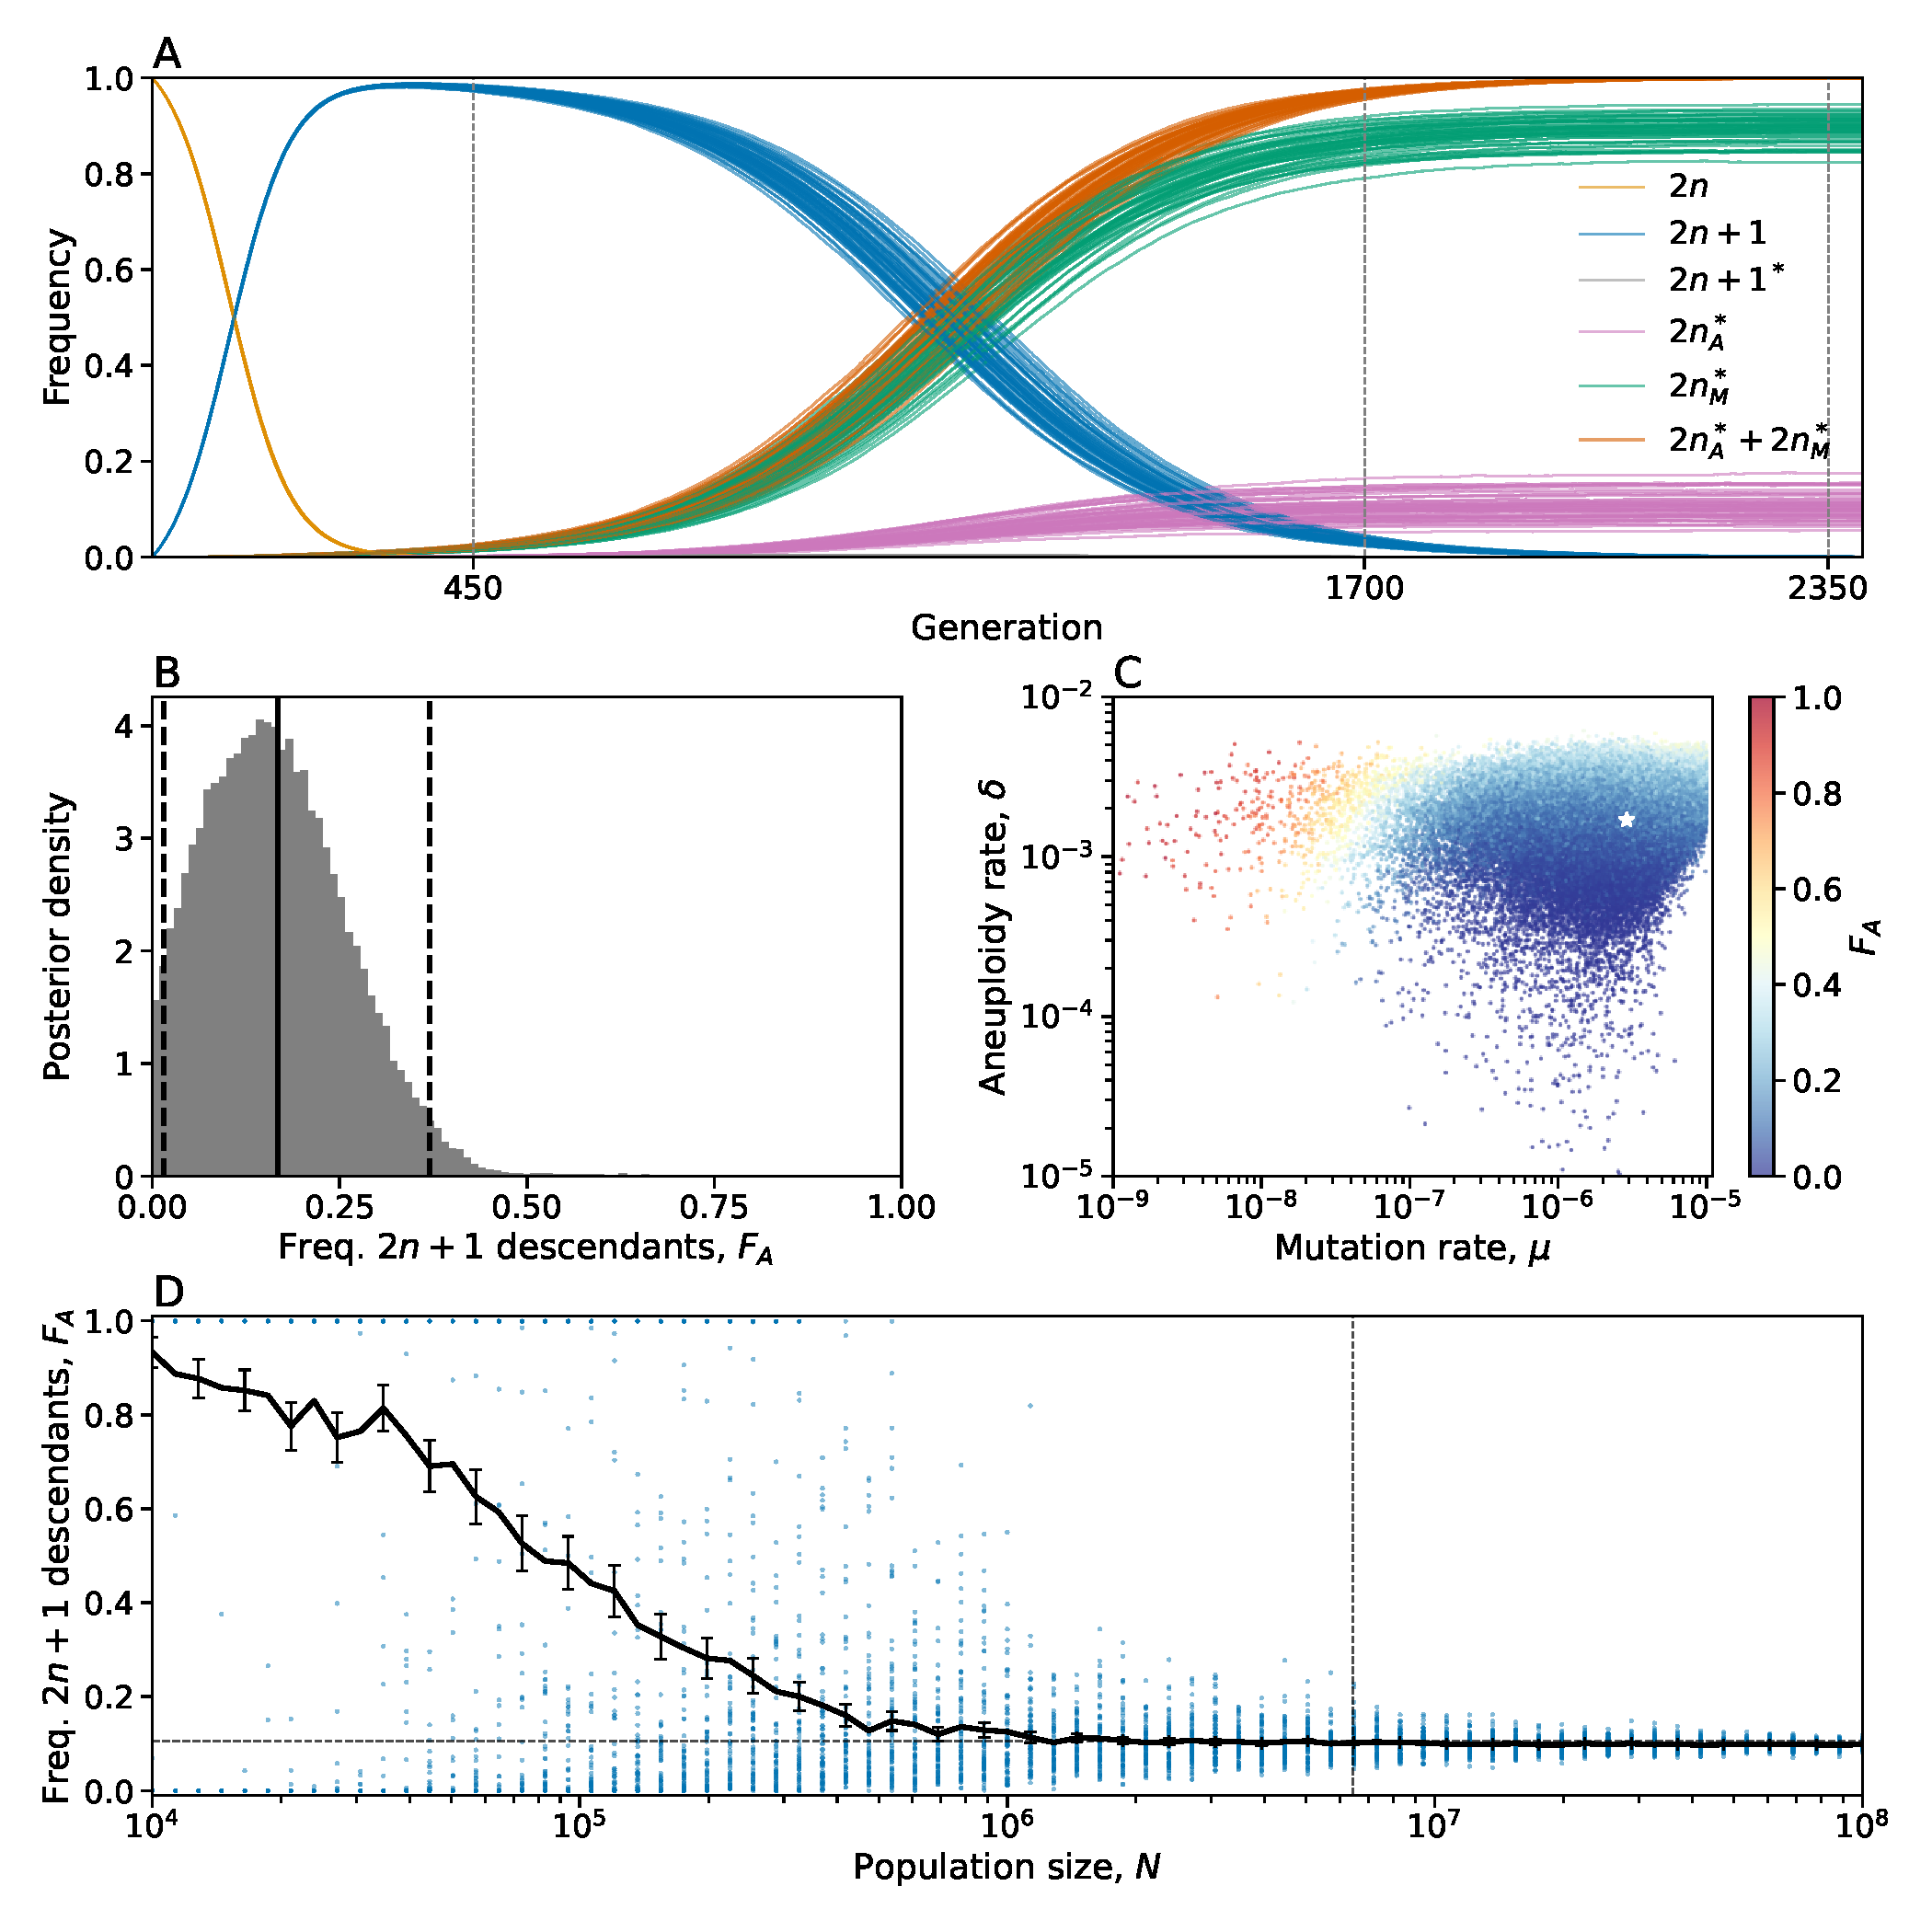
\includegraphics[width=0.8\textwidth]{../figures/FA.pdf}      
  \caption{
    \textbf{Predicted frequency of aneuploid-descended cells.}     
    \textbf{(A)} Posterior predicted genotype frequencies over time, including the source of \eumt: $2n^*_A$ arose from $2n+1$, whereas $2n^*_M$ arose directly from $2n$. Colored curves are 50 simulations using the MAP estimate parameters. Black dashed curves are the expected genotype frequencies without genetic drift (from a deterministic model). 
     See \Cref{fig:MAP_freq_dynamics_log} for log-log scale, in which the sequence of events is easier to observe.
    \textbf{(B)} Posterior distribution of $F_A$, the expected frequency of \eumt\ cells descended from \anwt\ cells, computed as the average frequency at the end of 100 simulations for 100,000 samples from the parameter posterior distribution.
    Solid and dashed lines show the mean and 95\% CI.
	\textbf{(C)} $F_A$ values (color coded) from panel B, with their corresponding mutation rate $\mu$ on x-axis and aneuploidy rate $\delta$ on the y-axis.
	White star shows the MAP estimate. See also \Cref{fig:posterior_FA_supp}.
	\textbf{(D)} $F_A$ as a function of the population size, $N$, in posterior predictions with MAP parameters. Markers show $F_A$ in 250 simulations per population size. Error bars show mean $F_A$ with 95\% CI (bootstrap, $n=10,000$). Vertical dashed line for population size in the experiment, $6.425\cdot10^6$. Horizontal line for $F_A^{MAP}=0.106$. 
	\textbf{(E)} Population mean fitness in a model without drift using MAP estimate parameters. Solid lines for mean fitness with aneuploidy ($\delta>0$), where the population reaches adaptation (mean fitness at 99.99\% of maximum value) at generation 1,802. Dashed lines for mean fitness without aneuploidy ($\delta=0$), where the population adapts much earlier, at generation 535.
     }
  \label{fig:FA}
\end{figure}
%%%%%%%%%%%%%%%%%%%%%%%%%%%%%%%%%%%%%%%%%%%%


\paragraph{Genetic instability in aneuploid cells.}
It has been suggested that aneuploidy increases genetic instability~\citep{Sheltzer2011b, Ippolito2021b}. Therefore, we inferred model parameters under the assumption that the mutation rate increases in aneuploid cells by a factor $\tau$ = 1, 33/32 (due to an additional chromosome), 2, 5, 10, or 100 (due to genetic instability).
We found that the posterior distribution was similar for $\tau=$1, 33/32, 2, and 5 (\Cref{fig:tau}).
%% generated with MAP-and-hdi.ipynb
With $\tau=100$, the estimated mutation rate was about 7-8-fold lower compared to $\tau=1$ ($\mu=4.094\cdot10^{-7}\ [6.252\cdot10^{-8}-6.046\cdot10^{-7}]$) and the aneuploidy rate was about 2-3-fold lower ($\delta=0.744\cdot10^{-3}\ [0.506\cdot10^{-3}-1.827\cdot10^{-3}]$). 
With $\tau=10$, the estimated mutation rate was only slightly lower compared to $\tau=1$ ($\mu=1.67\cdot10^{-6}\ [2.836\cdot10^{-8}-2.245\cdot10^{-6}]$). 
WAIC (lower is better, see Methods) is lowest for $\tau=33/32$ and $\tau=1$ (\Cref{table:WAIC}).
Therefore, our results do not support an increase in mutation rate in aneuploid cells. This may be because, unless the increase is strong ($\tau \ge 10$), it does not seem to affect our inference; or because chromosome III is one of the smallest chromosomes \citep{Gilchrist2019}.
We also checked the differences in genotype frequency dynamics for different $\tau$ values. We observe $\tau=100$ could be distinguished if accurate data was available for the waiting time until the frequency of \euwt\ to decrease below 95\%~(\Cref{fig:tau-plots}A) or for waiting time for the frequency of \anwt\ to either reach or go below 95\%~(\Cref{fig:tau-plots}B).


%%%%%%%%%%%%%%%%%%%%%%%%%%%%%%%%%%%%%%%%%%%%%%%%%%%%%%%%%%%%
% Discussion
\section*{Discussion}

In a landmark study on the role of chromosome duplication in adaptive evolution, 
\citet{Yona2012} found that a chromosome III trisomy was acquired by \yeast populations evolving under heat stress, only to be later replaced by euploid mutant cells that carry "refined" solutions to the stress. 
Additionally, such a replacement also occurred when they initiated evolutionary experiments with a population in which all cells carry a chromosome III trisomy.
They hypothesized that the euploid mutant cells evolved by heat-resistance mutations in aneuploid cells followed by reversion of trisomy due to a chromosome loss event. 

If indeed the evolved euploid population is descended from the aneuploid population, then mutant alleles that were common in the aneuploid populations should also be common in the evolved euploid population.
However, we found that this is not the case (\Cref{fig:mutation_frequencies}): mutant allele frequencies in the aneuploid and euploid populations are negatively correlated, such that common alleles in the former are rare in the later. 
Furthermore, we developed an evolutionary genetic model of adaptive evolution by aneuploidy and mutation (\Cref{fig:models}), fitted it to the experimental results of \citet{Yona2012}, and used it to predict the genotype frequency dynamics.
The model predicted that only about 10-15\% of the evolved euploid population descended from aneuploid cells--that is, the majority of the euploid population are not descended from aneuploid cells, but rather are direct descendants of the ancestral wild-type population (\Cref{fig:FA}).

This happens despite aneuploidy reaching a high frequency in the population (>95\%). 
Conventional wisdom might suggest that once the aneuploid genotype \anwt\ reaches high frequency, it will have a better chance at producing "refined" solutions via mutations, and its descendants will come to dominate the population: the frequency of \eumtA\ (which arises from \anmt) will be higher than the frequency of \eumtM\ (which arises directly from \euwt).

So how does \eumtM\ prevail?
Initially, the supply rates of \anwt\ and \eumtM\ are $N \delta \approx 11,000$ and $N \mu \approx 19$, respectively (assuming MAP parameter estimates). 
Therefore, both genotypes are expected to appear immediately at the beginning of the experiment (\Cref{fig:MAP_freq_dynamics_log}).
However, \anwt\ appears at a much higher frequency as $\delta \gg \mu$ by 2-3 orders of magnitude.
After they first appear, \eumtM\ has higher fitness.
But as long as the frequency of \euwt\ is high, the supply rate of \anwt\ is higher than that of \eumtM, again due to $\delta \gg \mu$. 
However, supply rates of both genotypes decreases with the frequency of \euwt.
Therefore, when the latter decreases, mainly due to the increase in the frequency of \anwt, both supply rates diminish.
At this stage, the higher fitness of \eumtM\ comes into play and it starts to take over the population, which is mainly composed of \anwt.
For the aneuploid lineage to compete with the mutant lineage, it must produce \eumtA\ via a mutation followed by chromosome loss.
Although this is a stochastic process (due to drift), our results show that the time until \eumtA\ reaches a frequency of ~0.1\% is roughly 450 generations, without much variation (intersection of purple lines and vertical dashed line in \Cref{fig:MAP_freq_dynamics_log}).
However, by that time \eumtM\ is already at a roughly 10-fold higher frequency (1.86\%), and since both mutants have the same fitness, their relative frequency remains roughly the same until the end of the experiment. 

% population size
\paragraph{Predictions for small populations.}
We examined the effect of the population size, $N$, on the frequency of \anwt\ descendants in the evolved population, $F_A$.
We found that $F_A$ is expected to decrease as the population size increases (\Cref{fig:FA}D), ranging from about 90\% when the population size is 10,000, to about 10\% when the population size is above 1,000,000 (less than the experimental population size, which was 6,425,000). 
Thus, our model provides a testable prediction: if the experiment was repeated under a lower population size (via stronger daily dilutions or in a smaller volume), than the fraction of the population descending from aneuploid cells would be much higher.

% mean fitness
\paragraph{Aneuploidy delays rather than facilitates adaptation.}
An additional interesting result of our study is that aneuploidy increases, rather than decreases, the adaptation time (\Cref{fig:FA}E). 
This happens despite the fact that the mean fitness initially increases faster in the presence of aneuploidy (\Cref{fig:FA}E). 
This is because once \anwt\ is common, selection for the mutant strain (\anmt\ or \eumt) is weaker compared to when \eumt\ competes directly with \euwt.

% parameter estimates
\paragraph{Rate and fitness effect of aneuploidy and mutation.}
We inferred the rates of aneuploidy and mutation and their effects on fitness. 
We estimate that the aneuploidy rate (i.e., number of chromosome gains per generation) is $1.7 \cdot 10^{-3}$, higher than a previous estimate of $6.7 \cdot 10^{-6}$~\citep{Zhu2016}. This may be due to genetic instability caused by heat stress~\citep{Chen2012a}.
In addition, we find no evidence for increased mutation rates in aneuploid cells. 
Previous empirical studies have suggested that genetic instability (e.g., elevated mutation rates) in aneuploid cells is due to stress associated with the aneuploid state~\citep{Bouchonville2009, Chen2012b, Zhu2012, Ippolito2021b}.
However, in the experiment of \citet{Yona2012}, both the wild-type and the aneuploid were under heat stress, which may explain why we did not find evidence for an increased mutation rate.

% TODO caveats - MP

% Conclusions
\paragraph{Conclusions.}
Here, we tested the hypothesis that aneuploid cells are an evolutionary "stepping stone", or adaptive intermediate, between wild-type euploid cells and mutant euploid cells. 
Our results suggest that, although it seems the population goes from euploid to aneuploid and back, this is not the case at the individual level. We estimate that only about 10-15\% of the euploid cells descended from aneuploid cells, whereas the rest are direct descendants of the wild-type euploid cells.
This surprising result reinforces the importance of models when making interpretations on evolutionary processes, and emphasizes the unintuitive outcomes of clonal interference during adaptive evolution.


%%%%%%%%%%%%%%%%%%%%%%%%
% Models and Methods
\section*{Models and Methods}

%%%%%%%%%%%%%%%%%%%%%%%%
\paragraph{DNA sequencing.}
Whole-genome sequencing of the ancestral diploid strain (\euwt) was performed on a sample generated from a single colony of the ancestor.
Whole-genome sequencing of the four evolving populations ($H2$ after 450 and 2,350 generations, and $H4$ after 450 and 1,700 generations) was performed at the population level.
A liquid sample from each evolving population was taken for sequencing from each culture as it grows under the same conditions as the lab evolution experiments (YPD at \SI{39}{\celsius}).
DNA was purified from the collected cells for each population and downstream deep sequencing was performed according to the Illumina protocol for amplicon sequencing. 

\paragraph{Evolutionary genetic model.}
We model the evolution of a population of cells using a Wright-Fisher model~\citep{Otto2007}, assuming a constant effective population size $N$, non-overlapping generations, and including the effects of natural selection, genetic drift, aneuploidy, and mutation. 
We focus on beneficial genetic modifications, neglecting the effects of deleterious and neutral mutations or karyotypic changes.
The model allows for a single aneuploid karyotype (e.g., chromosome III duplication) and a single mutation to accumulate in the genotype.
Thus, the model follows four genotypes~(\Cref{fig:models}): euploid wild-type, \euwt, the initial genotype; 
euploid mutant, \eumt, with the standard karyotype and a single beneficial mutation; 
aneuploid wild-type, \anwt, with an extra chromosome, i.e., following chromosome duplication; and
aneuploid mutant, \anmt, with and extra chromosome and a beneficial mutation. 

Transitions between the genotypes occur as follows~(\Cref{fig:models}): Beneficial mutations from \euwt\; to \eumt\; and from \anwt\; to \anmt\; occur with probability $\mu$, the mutation rate. We neglect back-mutations (i.e., from \eumt\; to \euwt\; and from \anmt\; to \anwt).
Aneuploidy is formed by chromosome mis-segregation, so that cells transition from \euwt\; to \anwt\; and from \anmt\ to \eumt\ with probability $\delta$, the aneuploidy rate. That is, we assume chromosomes are gained and lost at the same rate, and we neglect events that form a less-fit genotype (i.e., \anwt\; to \euwt\; and \eumt\; to \anmt).

In the experiment by \citet{Yona2012}, the population was grown every day from $1.6 \cdot 10^6$ cells until reaching stationary phase and then diluted 1:120.
Thus, we set the population size to $N=6.425 \cdot 10^6$, the harmonic mean of $\{2^k \cdot 1.6 \cdot 10^6\}_{k=0}^{7}$~\citep{Crow1970}.
The initial population has $N$ cells with genotype \euwt. 
The effect of natural selection on the frequency $f_i$ of genotype $i = 2n, 2n+1, 2n+1^*, \text{or } 2n^*$ is given by
    \begin{equation} \label{eq:selection-single} 
      f^s_i = \frac{f_i w_i}{\bar{w}} \;,
    \end{equation}
where $w_i$ is the fitness of genotype $i$ and $\bar{w} = \sum_{j}{f_j w_j}$ is the population mean fitness.
The effect of mutation and aneuploidy on genotype frequencies is given by
    \begin{equation} \label{eq:mutation-aneuploidy-single}
    \begin{aligned}
      &f^m_{2n} &=&\; (1 - \delta - \mu) f^s_{2n}  \;,\\
      &f^m_{2n+1} &=&\; \delta f^s_{2n} + (1 - \mu) f^s_{2n+1}  \;,\\
      &f^m_{2n+1^*} &=&\; \mu f^s_{2n+1} + (1-\delta) f^s_{2n+1^*}  \;,\\
      &f^m_{2n^*} &=&\; \mu f^s_{2n} + \delta f^s_{2n+1} + f^s_{2n^*}  \;.
    \end{aligned}
    \end{equation}
Finally, random genetic drift is modeled using a multinomial distribution~\citep{Otto2007},
    \begin{equation} \label{eq:drift-single}
      \vec{f'} \sim \frac{1}{N} \cdot \mathit{Mult}(N,\ \vec{f^m}) \;,
    \end{equation}
where $\vec{f^m}=(f^m_{2n}\ ,\ f^m_{2n+1}\ ,\ f^m_{2n+1^*}\ ,\ f^m_{2n^*})$ are the frequencies of the genotypes after mutation and aneuploidy, $\vec{f'}$ are the genotype frequencies in the next generation, and $Mult(N,\ \vec{f})$ is a multinomial distribution parameterized by the population size $N$ and the genotype frequencies $\vec{f}$.
Overall, the change in genotype frequencies from one generation to the next is given by the transformation $f_i \to f'_i$.

\paragraph{Empirical data for model inference.}

We use the results of evolutionary experiments reported by \citet{Yona2012}.
In their heat-stress experiment, four populations of \yeast evolved under \SI{39}{\celsius}. Aneuploidy fixed in all four population in the first 450 generations. Hereafter, fixation or elimination of a genotype \emph{by generation $t$} means that more than 95\% or less than 5\% of the population carry the genotype at generation $t$, and possibly earlier. 
From re-analysis of data not published in the original paper, aneuploidy did not fix before at least 200 generations elapsed.
The experiment continued with two populations, in which aneuploidy was eliminated by generation 1,700 and 2,350 while still under the same conditions of elevated heat (\SI{39}{\celsius}).


\paragraph{Likelihood function.} 
Because our model, just like the Wright-Fisher model, is non-linear and stochastic, computing the distribution of fixation time $T(g)$ of genotype $g$ for use in the likelihood function is intractable (it is even hard to use a diffusion-equation approximation due to the model having multiple genotypes, rather than just two).
We overcome this problem by approximating the likelihood using simulations. We simulate 1,000 experiments per parameter vector $\theta = (\mu, \delta, s, b, c)$, resulting in a set of simulated observations $\tilde{\vec X} = \{\tilde{X}_i\}_{i=1}^{1000}$. We then compute the approximate likelihood,
\begin{equation}\begin{aligned}
\label{eq:heatstress-likelihood}
\likelihood(\theta) = &\ P^4(200 \le T(2n+1) \le 450) \cdot 
	\Big[1 - \\
	&	P_{\tilde{\vec X}}^4\big(!\{T(2n^*)<1700\} \mid 200 \le T(2n+1) \le 450\big)- \\
	&	P_{\tilde{\vec X}}^4\big(!\{1700 < T(2n^*) < 2350\} \mid 200 \le T(2n+1) \le 450\big)+ \\
	&	P_{\tilde{\vec X}}^4\big(!\{T(2n^*)<1700\} \land !\{1700 < T(2n^*) < 2350\} \mid 200 \le T(2n+1) \le 450\big) 
	\Big]\;,
\end{aligned}\end{equation}
where $!\{\ldots\}$ is the "logical not" operator, $P^4(\ldots)$ is the 4th power of $P(\ldots)$, and all probabilities $P_{\tilde{\vec X}}(\ldots)$ are approximated from the results of the simulations $\tilde{\vec X}$. For example, $P_{\tilde{\vec X}}\big(!\{T(2n^*)<1700\} \mid 200 \le T(2n+1) \le 450\big)$ is approximated by taking simulations in which \anwt\; fixed before generation 450 but not before generation 200, and computing the fraction of such simulations in which \eumt\; did not fix by generation 1,700, and hence aneuploidy did not extinct before generation 1,700.
\Cref{fig:seeds} compares results with less and more simulated experiments, demonstrating that 1,000 simulations are likely sufficient.
 
For a model without aneuploidy (that is, when the aneuploidy rate is fixed at zero, $\delta=0$), we disregard the increased expression in chromosome III and the growth advantage measured in generation 450, and focus on the growth advantage measured in later generations, presumably due to a beneficial mutation. 
Therefore, the likelihood is approximated by
\begin{equation}\begin{aligned}
\label{eq:heatstress-noaneuploidy-likelihood}
\likelihood_{!}(\theta) = &\ 
	1 - 
	P_{\tilde{\vec X}}^4\big(!\{T(2n^*)<1700\}\big) - \\
&	P_{\tilde{\vec X}}^4\big(!\{1700 < T(2n^*) < 2350\}\big) + \\
&	P_{\tilde{\vec X}}^4\big(!\{T(2n^*)<1700\} \land !\{1700 < T(2n^*) < 2350\}\big)
\;.
\end{aligned}\end{equation}

\paragraph{Parameter inference.} To infer model parameters, we use approximate Bayesian computation with a sequential Monte-Carlo scheme, or ABC-SMC~\citep{Sisson2009}, implemented in the \texttt{pyABC} Python package~\citep[\href{https://pyabc.readthedocs.io}{pyabc.readthedocs.io}]{Klinger2018}.
This approach uses numerical stochastic simulations of the model to infer a posterior distribution over the model parameters. It is a method of likelihood-free, simulation-based inference~\citep{Cranmer2020}, that is, for estimating a posterior distribution when a likelihood function cannot be directly computed. It is therefore suitable in our case, in which the likelihood function can only be approximated from simulations, and cannot be directly computed. 

The ABC-SMC algorithm employs sequential importance sampling over multiple iterations~\citep{Toni2009, Klinger2017, Syga2021}.
In iteration $t$ of the algorithm, a set of parameter vectors, $\{\theta_{i,t}\}_{i=1}^{n_t}$, also called \emph{particles}, are constructed in the following way.
A proposal particle, $\theta^*$, is sampled from a proposal distribution, and is either accepted or rejected, until $n_t$ particles are accepted.
The number of particles, $n_t$, is adapted at every iteration $t$ using the adaptive population strategy~\citep[\href{https://pyabc.readthedocs.io}{pyabc.readthedocs.io}]{Klinger2018}.
For $t=0$, the proposal particle is sampled from the prior distribution, $p(\theta)$.
For $t>0$, the proposal particle is sampled from the particles accepted in the previous iteration, $\{\theta_{i,t-1}\}_{i=1}^{n_{t-1}}$, each with a probability relative to its weight $W_{t-1}(\theta_{i,t-1})$ (see below). The proposal particle is then perturbed using a kernel perturbation kernel, $K_t(\theta^* \mid \theta)$ where $\theta$ is the sample from the previous iteration.
Then, a set of synthetic observations $\tilde{\vec X}^*$ is simulated, and the proposal particle $\theta^*$ is accepted if its approximate likelihood (\cref{eq:heatstress-likelihood}) is high enough, $\likelihood(\theta^*)>1-\epsilon_t$ (or more commonly, if $1-\likelihood(\theta^*) < \epsilon_t$), where $\epsilon_t>0$ is the \emph{acceptance threshold}, as higher values of $\epsilon_t$ allow more particles to be accepted. 
The acceptance threshold $\epsilon_t$ is chosen as the median of the $1-\likelihood(\theta)$ of the particles accepted in the previous iteration, $t-1$, and $\epsilon_0=0.01$. 
For each accepted particle $\theta_{i,t}$ a weight $W_t(\theta_{i,t})$ is assigned: for $t=0$, $W_0(\theta_{i,0})=1$, and for $t>0$, 
$W_t(\theta_{i,t}) = p(\theta_{i,t}) / \sum_{i=1}^{n_{t-1}}{W_{t-1}(\theta_{i,t-1}) K_t(\theta_{i,t}, \theta_{i,t-1})}$, where $p(\theta)$ is the prior density of $\theta$ and $K_t(\theta', \theta)$ is the probability of a perturbation from $\theta$ to $\theta'$.
$K_t(\theta' \mid \theta)$ is a multivariate normal distribution, fitted at iteration $t$ to the particles from the previous iteration, \{$\theta_{i,t-1}\}_{i=1}{n_{t-1}}$, and their weights, $\{W(\theta_{i,t-1})\}_{i=1}^{n_{t-1}}$.

Acceptance is determined according to the approximate likelihood~(\cref{eq:heatstress-likelihood}), which has a maximum value of $\likelihood_{max}=0.875$ (giving a minimal value of $\epsilon_{min}=0.125$). We terminated the inference iterations when the change in $\epsilon$ value from one iteration to the next was small.
With our standard prior and model, we reached $\epsilon=0.13$ (or $\likelihood=0.87$) after six iterations, with $n_6=982$ accepted parameter vectors and effective sample size ESS=651 (\Cref{fig:convergence}). Running the inference algorithm with different initialization seeds and less or more simulations for approximating the likelihood produced similar posterior distributions~(\Cref{fig:seeds}). 

After producing a set of weighted particles from the the posterior distribution using the above ABC-SMC algorithm, we approximate the posterior using kernel density estimation (KDE) with Gaussian kernels. We truncate the estimated posterior to avoid positive posterior density for values with zero prior density. The MAP (maximum a posteriori) estimate is computed as the the maximum of the estimated joint posterior density. We then draw $5,000,000$ samples from the posterior distribution to compute the HDI (highest density interval) and draw $50,000$ samples to visualize the posterior distribution with histograms.

\paragraph{Model comparison.} 
We examine several versions of our evolutionary models, e.g. without aneuploidy or with increased mutation rate in aneuploid cells, as well as several different prior distributions (see below).
To compare these, we plot posterior predictions: for each model we execute $10,000$ simulations using the MAP parameter estimates and plot the distributions of time to fixation of \eumt, one of key properties of the model likelihood. These plots visualize the fit of each model to the data. 
Also, for similar models we plot the marginal and joint posterior distributions of the parameters; if these are similar, we consider the models interchangeable. We validate this by comparing HDI (highest density interval) of posterior distributions.

Where posterior plots are very similar and the number of parameters is the same, we use WAIC, or the widely applicable information criterion ~\citep{gelman2013bayesian}, defined as
\begin{equation} \label{eq:WAIC}
\begin{aligned}
\mathit{WAIC}(\theta) &\ =\ 
-2\log\mathbb{E}[\likelihood(\theta)]\ +\ 2\mathbb{V}[\log\likelihood(\theta)]
\end{aligned}
\end{equation}
where $\theta$ is a parameter vector, and $\mathbb{E}[\cdot]$ and $\mathbb{V}[\cdot]$ are the expectation and variance taken over the posterior distribution, which in practice are approximated using 50,000 samples from the posterior KDE. We validated that upon resampling WAIC values do not significantly change and that differences in WAIC between models are preserved.
WAIC values are scaled as a deviance measure: lower values imply higher predictive accuracy~\citep{Kass1995}.
 
\paragraph{Prior distributions.} \label{par:prior}
We used informative prior distributions for $w_{\anwt}=1-c+b$, $w_{\anmt}=(1+s)(1-c)+b$ and $w_{\eumt}=1+s$, which we estimated from growth curves data from mono-culture growth experiments previously reported by \citet[Figs. 3C, 4A, and S2]{Yona2012}.
We used \texttt{Curveball}, a method for predicting results of competition experiments from growth curve data~\citep[\href{https://curveball.yoavram.com}{curveball.yoavram.com}]{Ram2019}. Briefly, \texttt{Curveball} takes growth curves of two strains growing separately in mono-culture and predicts how they would grow in a mixed culture, that is, it predicts the results of a competition assay.
From these predictions, relative fitness values can be computed. Because \texttt{Curveball} uses a maximum-likelihood approach to estimate model parameters, we were able to estimate a distribution of relative fitness values to be used as a prior distribution by sampling 10,000 samples from a truncated multivariate normal distribution defined by the maximum-likelihood covariance matrix~(\Cref{fig:growth-curves}).

We used growth curves of \euwt\ and \anwt\ in \SI{39}{\celsius} to estimate an informative prior distribution for $w_{\anwt}$~(\Cref{fig:growth-curves}-D, assuming $w_{\euwt}=1$).
In this prior distribution, we used the same prior for $w_{\anmt}$ and $w_{\eumt}$. 
To increase computational efficiency, we also assumed $w_\eumt>w_\anmt>w_\anwt>w_\euwt$; running the inference without this assumption produced similar results.
See \emph{supporting material} for an extended informative prior distribution that uses growth curves of \eumt\ and \anwt\ growing in \SI{39}{\celsius}; this prior distribution proved to be less useful.

As a control, we tested an uninformative uniform prior with $\mathit{U}(1,6)$, for (i) all $w_{\anwt}$, $w_{\anmt}$, $w_{\eumt}$, or (ii) only for $w_{\anmt}$, $w_{\eumt}$, using the above informative prior for $w_{\anwt}$. In these cases the inference algorithm failed to converge.
 
For the mutation rate, $\mu$, and aneuploidy rate, $\delta$, we used uninformative uniform priors, $\mu \sim \mathit{U}(10^{-9},10^{-5})$ and $\delta \sim \mathit{U}(10^{-6},10^{-2})$. A wider mutation rate prior, $\mu \sim \mathit{U}(10^{-9},10^{-3})$, produced similar results.


%%%%%%%%%%%%%%%%%%%%%%%%%%%%%%%%%%%%

% Acknowledgements
{\small
\section*{Acknowledgements}
We thank Yitzhak Pilpel, Orna Dahan, Lilach Hadany, Judith Berman, David Gresham, Shay Covo, Martin Kupiec, Uri Obolski, Daniel Weissman, and Tal Simon for discussions and comments.
This work was supported in part by 
the Israel Science Foundation~(ISF, YR 552/19),
the US--Israel Binational Science Foundation~(BSF, YR 2021276)
Minerva Stiftung center for Lab Evolution~(YR),
Minerva Stiftung short-term research grant~(MP).
}

\bibliographystyle{agsm}
\bibliography{ms.bib}

\newpage

\section*{Supplementary Material}
\beginsupplement % https://support.authorea.com/en-us/article/how-to-create-an-appendix-section-or-supplementary-information-1g25i5a/

\subsection*{Supplementary Analysis}
\label{sec:supp_analysis}

\paragraph{Sensitivity analysis.} 
Changing a single parameter while keeping the rest fixed at the MAP estimate produces a worse fit to the data~(\Cref{fig:sensitivity}).
Furthermore, we fitted models with a mutation rate fixed at $\mu=10^{-5}$, $10^{-6}$ and $10^{-7}$.
We inferred similar parameters estimates for the model with $\mu=10^{-6}$ compared to the model with a free $\mu$ parameter, in which the inferred mutation rate is $\mu \approx 3\cdot10^{-6}$.
Inference assuming $\mu=10^{-5}$ or $\mu=10^{-7}$ produced similar estimates except that the estimated aneuploidy rate, $\delta$, was higher, and assuming $\mu=10^{-7}$, the estimated fitness of \anwt\ was lower (\Cref{fig:mu}).

\paragraph{Extended informative prior distribution.}
In an extended informative prior distribution, we used additional growth curves of \eumt\; (\emph{refined} strain from \citet{Yona2012}) and \anwt\; in \SI{39}{\celsius} to estimate $w_{\eumt}/w_{\anwt}$~(\Cref{fig:growth-curves}L). The same distribution was used for $w_{\eumt}/w_{\anmt}$. 
Thus, our main informative prior uses a single prior distribution for fitness values of \anwt, \anmt, and \eumt, whereas the extended informative prior uses one distribution for \anwt, and another distribution for both \anmt\ and \eumt. 

% generated with alt-prior.ipynb
We estimated the parameters under this extended informative prior.
Inference took much longer to run but the posterior distribution seemed to converge, as it did not change much in the final iterations. 
The posterior predictive plot shows that inference with this extended prior produces a posterior distribution that fails to explain the empirical observations~(pink in Figure~\ref{fig:2n*-fixation}).
However, the inferred posterior distribution is considerably narrower (compare \Cref{fig:posterior,fig:posterior-alt}) and therefore parameter estimates are less variable.
The estimated mutation rate was much lower compared to the main informative prior, 
% generated with MAP-and-hdi.ipynb
with $\mu=2.474\cdot10^{-9}\ [2.423\cdot10^{-9}-2.612\cdot10^{-9}]$. Other parameter estimates are: $\delta=2.705\cdot10^{-3}\ [2.094\cdot10^{-3}-3.094\cdot10^{-3}]$,
$w_{\anwt}=1.022\ [1.021-1.024]$,
$w_{2n+1^*}=1.052\ [1.05-1.054]$,
$w_{2n^*}=1.053\ [1.051-1.055]$, the latter two being much higher compare to the main informative prior. 
Notably, the mode of the posterior ratio $w_{\eumt}/w_{\anwt}=1.0009$ is much lower than the mode of the prior ratio of $1.033$ (\Cref{fig:growth-curves}H) and closer to the ratio of $1$ that we assume in the main informative prior.
Together with the posterior predictive results, we conclude that the main informative prior is preferable over the extended informative prior.


\paragraph{Model with transitions to less-fit genotypes}

We also estimated the parameters of a version of the model that includes transitions (mutation, chromosome loss and gain) to less-fit genotypes (e.g., \eumt\ to \anmt),
\begin{equation} \label{eq:mutation-aneuploidy-single}
    \begin{aligned}
      &f^m_{2n} &=&\; (1 - \delta - \mu) f^s_{2n} + \delta f^s_{2n+1} + \mu f^s_{2n^*} \;,\\
      &f^m_{2n+1} &=&\; \delta f^s_{2n} + (1 - \delta - \mu) f^s_{2n+1} + \mu f^s_{2n+1^*}  \;,\\
      &f^m_{2n+1^*} &=&\; \mu f^s_{2n+1} + (1 - \delta - \mu) f^s_{2n+1^*} + \delta f^s_{2n^*}  \;,\\
      &f^m_{2n^*} &=&\; \mu f^s_{2n} + \delta f^s_{2n+1^*} + (1 - \delta - \mu) f^s_{2n^*}  \;.
    \end{aligned}
    \end{equation}

The inferred values are slightly different.
% with back transitions MAP-and-hdi.ipynb
The estimated mutation rate, $\mu=1.036\cdot10^{-7}\ [8.01\cdot10^{-8}-1.339\cdot10^{-7}]$, corresponds to a mutation target size of $\sim 300-500$, assuming the mutation rate per base pair is roughly $2\cdot10^{-10}$ (ref.~\citep{Zhu2014}) or $3.3\cdot10^{-10}$ (ref.~\citep{Lynch2008}).
The estimated aneuploidy rate, $\delta=2.358\cdot10^{-4}\ [1.766\cdot10^{-4}-2.837\cdot10^{-4}]$ is 5-35-fold higher than in previous studies: for chromosome III in diploid \yeast, \citet{Zhu2014} estimated $6.7\cdot10^{-6}$ chromosome gain events per generation, and \citet{Kumaran2013} estimate $3.0-4.3\cdot10^{-5}$ chromosome loss events per generation (95\% confidence interval).
The estimated fitness values are 
$w_{\anwt}=1.024\ [1.023-1.025]$,
$w_{\anmt}=1.025\ [1.024-1.026]$,
$w_{\eumt}=1.032\ [1.031-1.033]$, all relative to the fitness of \euwt, which is set to $w_{\euwt}=1$. 
Thus, we can infer that the cost of trisomy is $c = w_{\eumt}-w_{\anmt} = 0.007$ (or 0.7\%) and the benefit of trisomy is $w_{\anwt}-1-c=0.017$ (1.7\%), whereas the benefit of beneficial mutation is $w_{\eumt}-1=0.032$ (3.2\%).

We simulated genotype frequency dynamics using parameter samples from the posterior distribution, and computed the posterior distribution of $F_A$. 
The mean $F_A$ in this case is just 0.0189 [0.0004 - 0.1214 95\% CI], lower than without the transitions to less-fit genotypes. Here, $F_A$ is the sum of frequencies of both \eumtA\ and $2n+1^*_A$, which reaches a frequency of 0.0007. Out of 100,000 posterior samples, none had $F_A$ above 0.05 (i.e., 5\% of the population).


%%%%%%%%%%%%%%%%%%%%%%%%%%%%%%%%%%
\newpage
\subsection*{Supplementary Figures \& Tables}


% Fig Validation of posteriors
%% generated with diff-runs.ipynb
\begin{figure}[h]
    \centering
      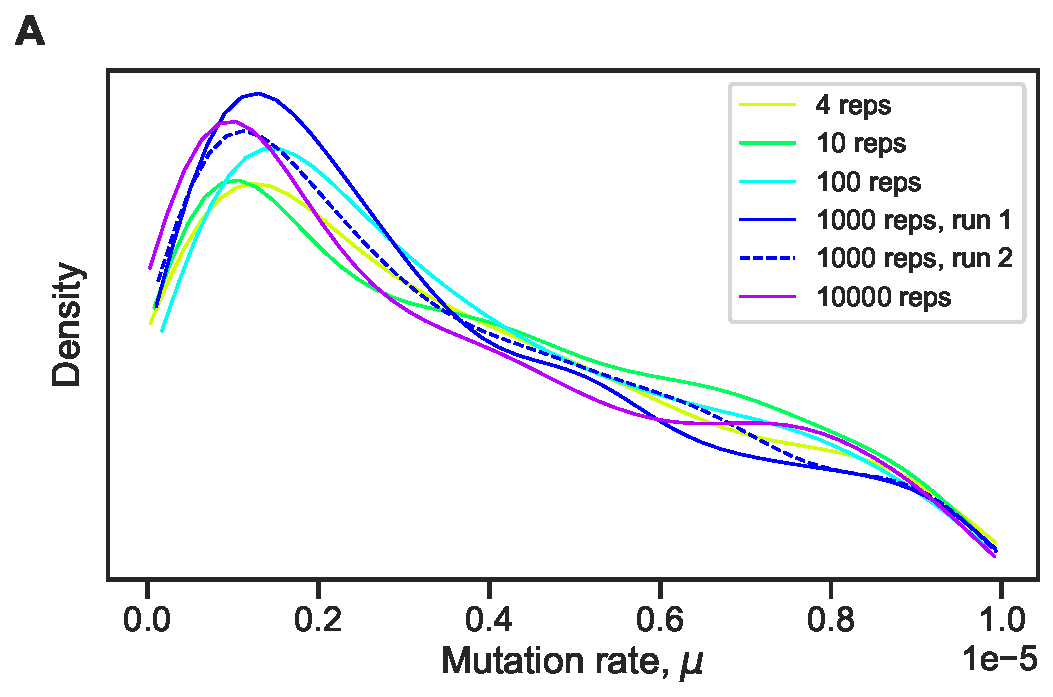
\includegraphics[width=0.45\textwidth]{../figures/runs-A.pdf}      
      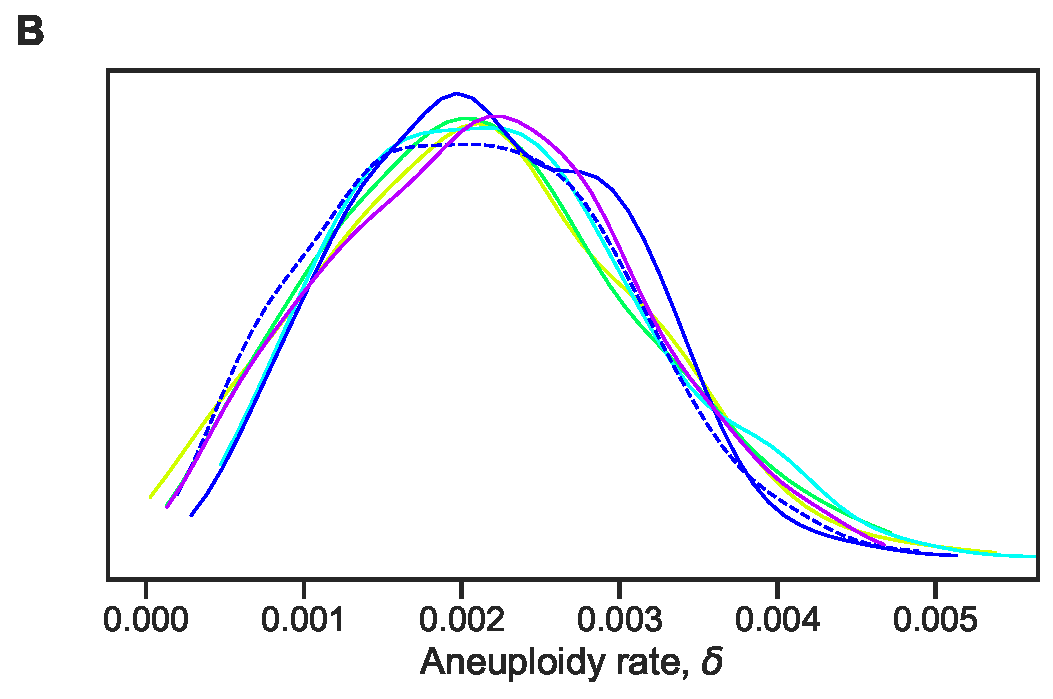
\includegraphics[width=0.45\textwidth]{../figures/runs-B.pdf}    
      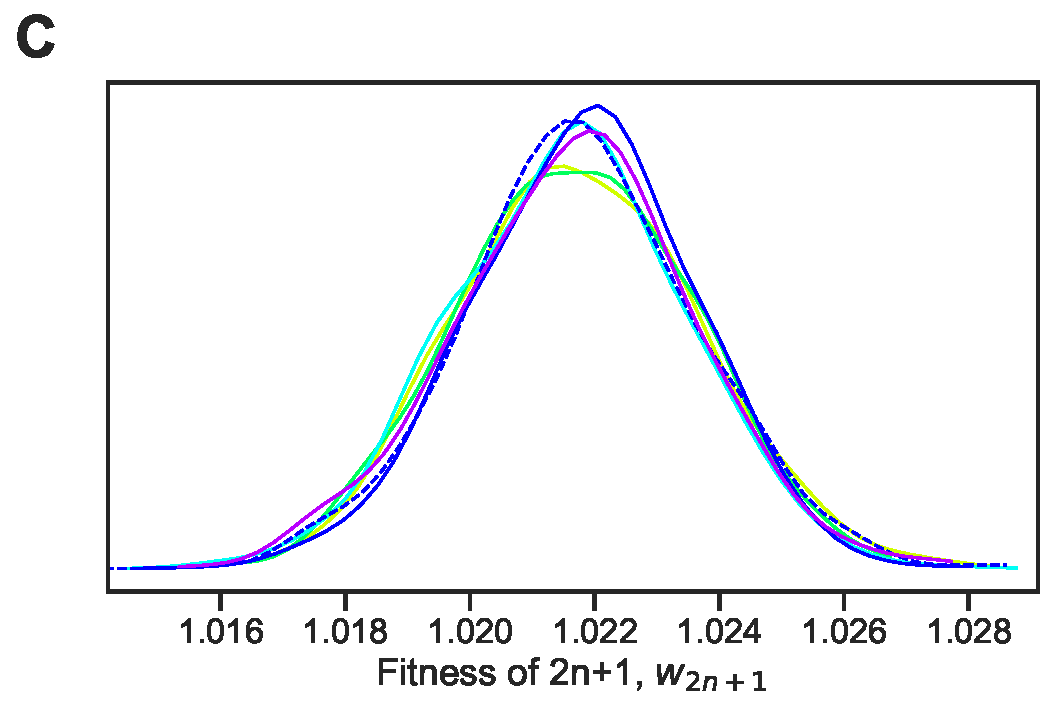
\includegraphics[width=0.325\textwidth]{../figures/runs-C.pdf}      
      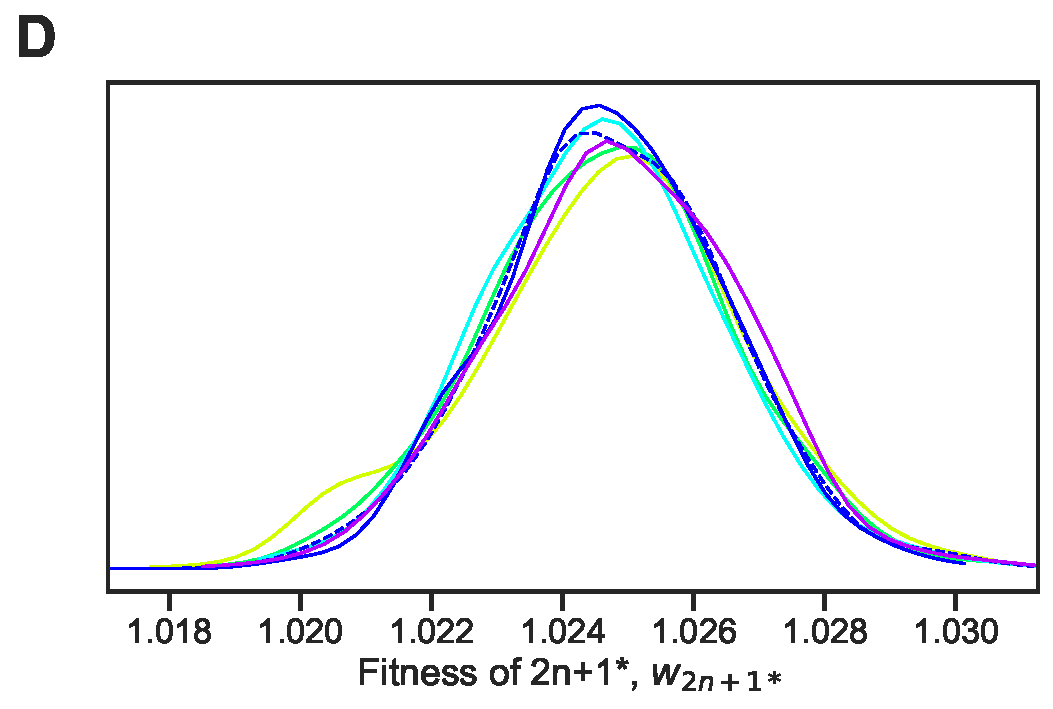
\includegraphics[width=0.325\textwidth]{../figures/runs-D.pdf}      
      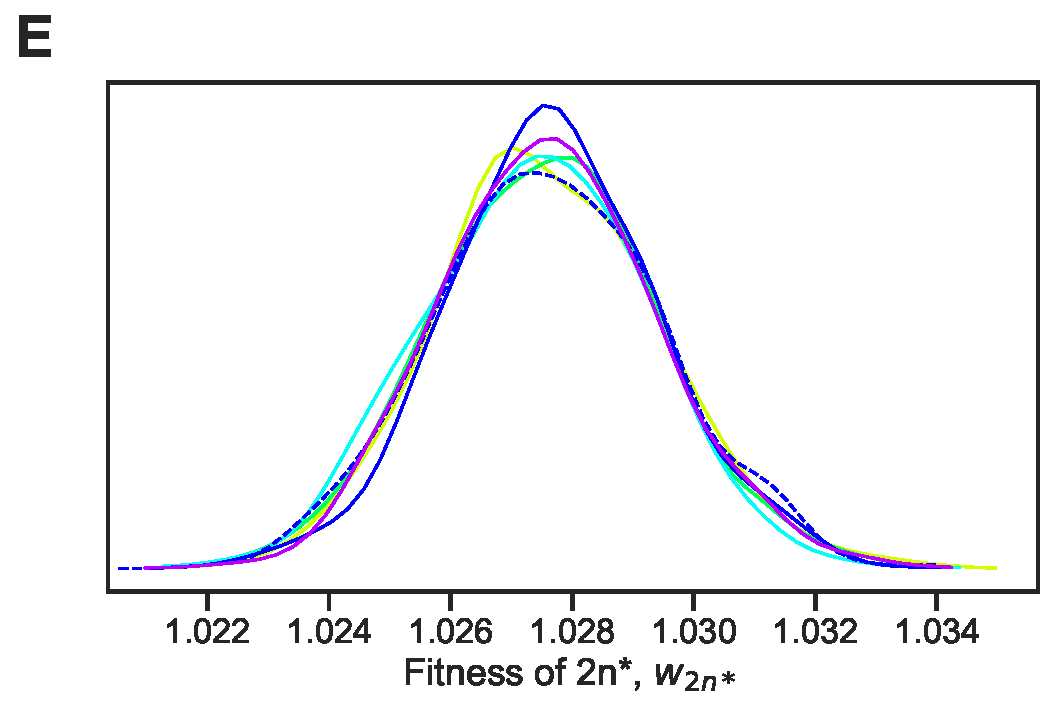
\includegraphics[width=0.325\textwidth]{../figures/runs-E.pdf} 
       \caption{
    \textbf{Posterior distribution validation.}
    The posterior distribution of model parameters is roughly the same regardless of the number of simulations (4-10,000 replicates) used to approximate the likelihood (\cref{eq:heatstress-likelihood}).
    } 
     
     \label{fig:seeds}
 \end{figure}



% Fig ABC iterations, convergence
%% generated with convergence.ipynb
\begin{figure}[p]

  \begin{subfigure}{1\textwidth}
    \centering
      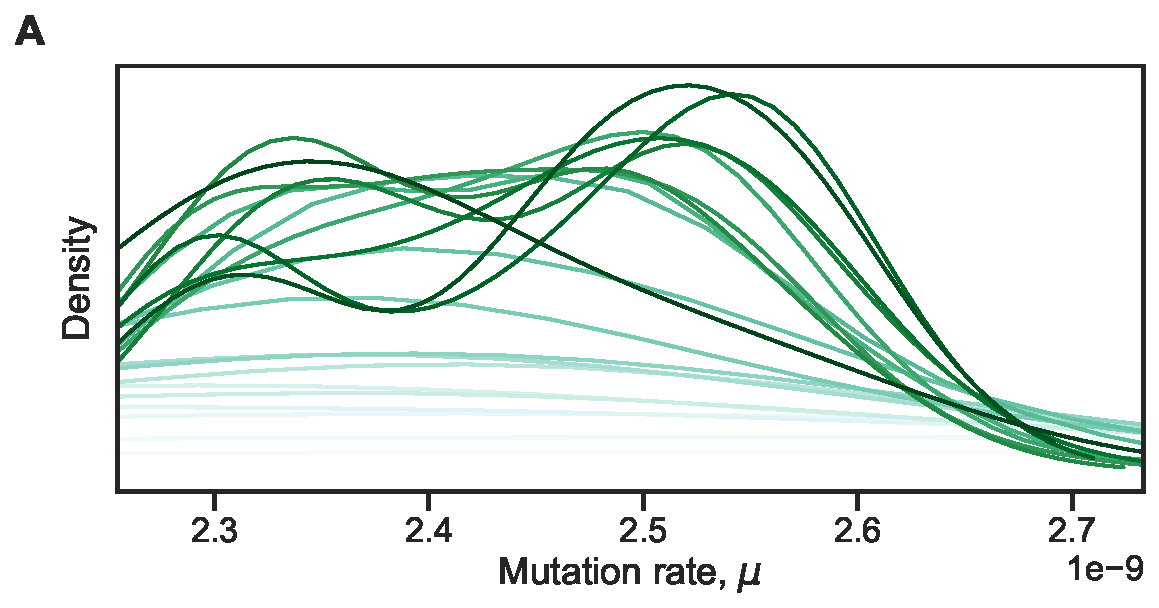
\includegraphics[width=0.45\textwidth]{../figures/convergence-p1_mr.pdf}      
      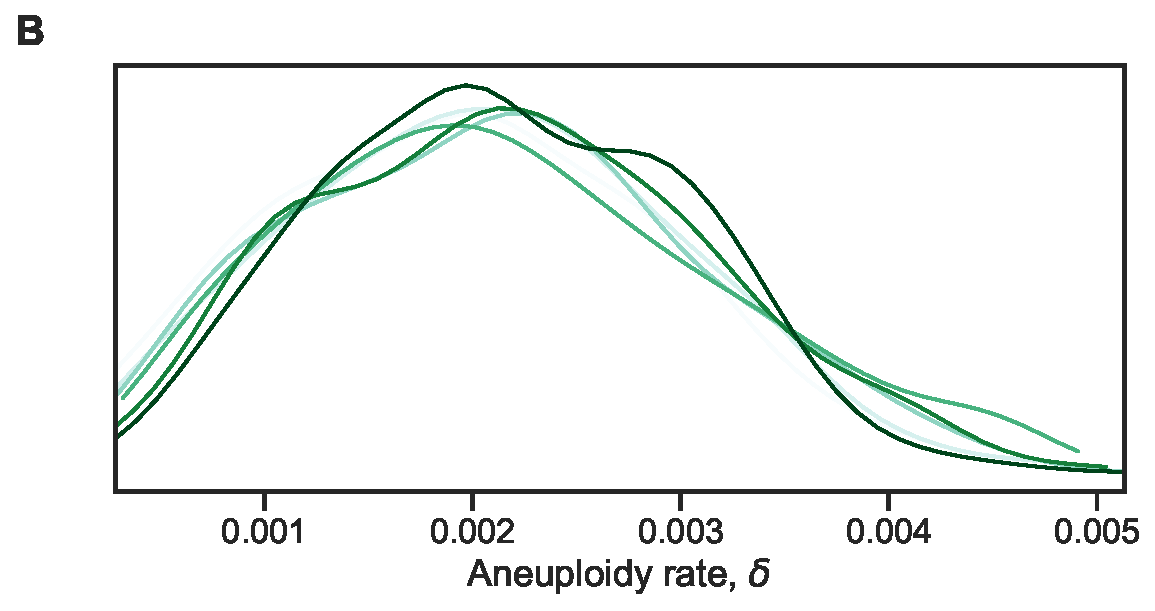
\includegraphics[width=0.45\textwidth]{../figures/convergence-p2_tr.pdf} \\     
      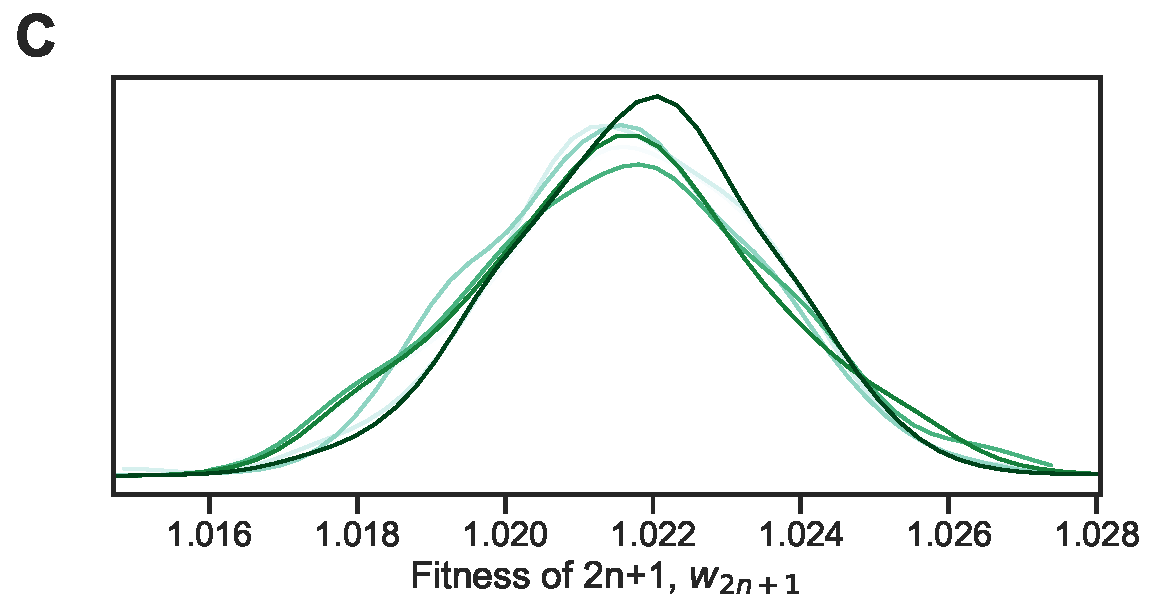
\includegraphics[width=0.325\textwidth]{../figures/convergence-p3_w1.pdf}      
      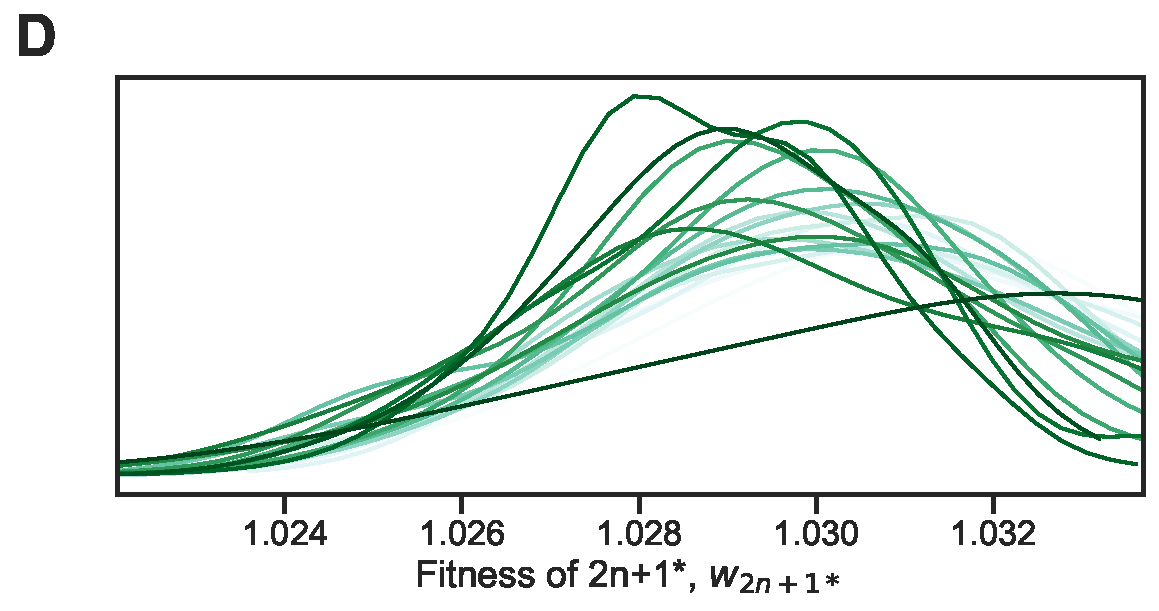
\includegraphics[width=0.325\textwidth]{../figures/convergence-p4_w2.pdf}      
      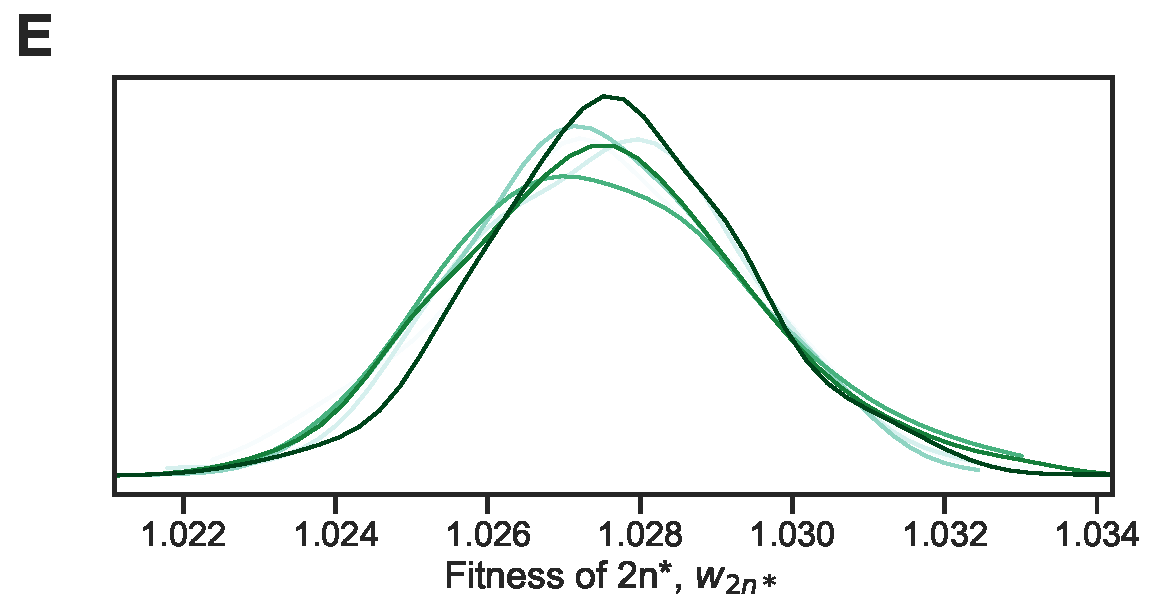
\includegraphics[width=0.325\textwidth]{../figures/convergence-p5_w3.pdf}      
     \label{fig:convergence-A}
    \end{subfigure}
    \\    
  \begin{subfigure}{1\textwidth}
  	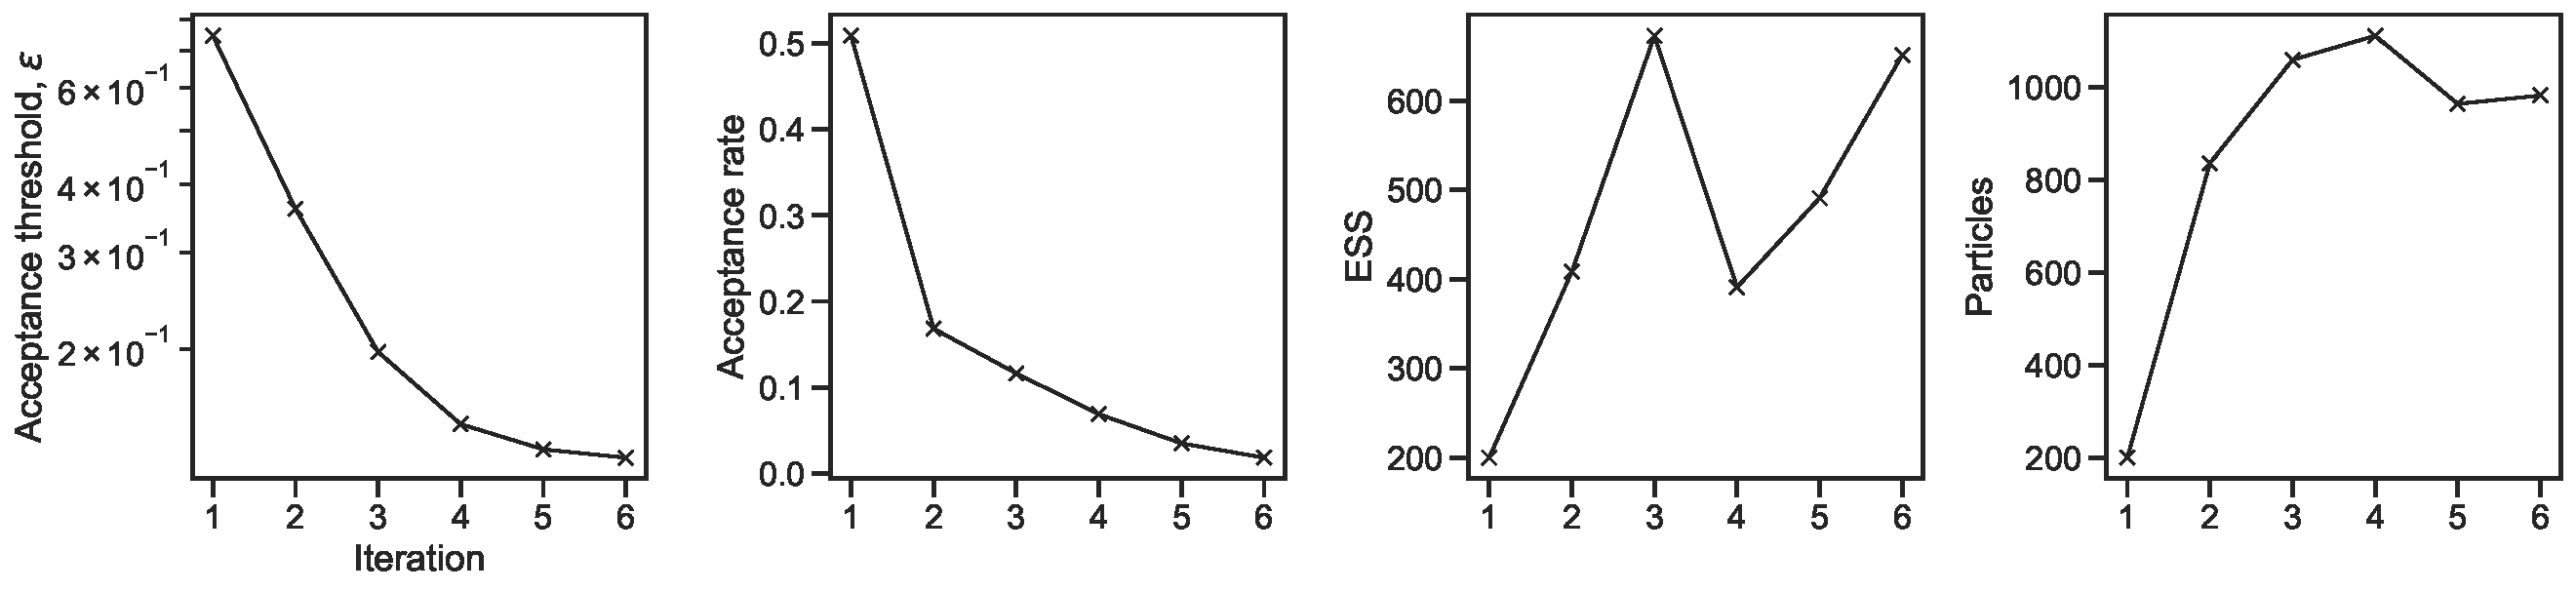
\includegraphics[width=\textwidth]{../figures/ess.pdf}
     \label{fig:convergence-B}
  \end{subfigure}
    \caption{
    \textbf{Inference convergence.} 
    The ABC-SMC algorithm was used to infer the model parameters. \textbf{(A-E)} The approximate posterior distributions of model parameters at each iteration of the ABC-SMC algorithm demonstrates convergence, as the posterior did not significantly change after the first iteration, $t=1$.
    \textbf{(F-I)} ABC-SMC measures of convergence. After iteration number 6, the acceptance threshold was $\epsilon=0.13$ (i.e., $\likelihood=0.87$, \cref{eq:heatstress-likelihood}), the acceptance rate was $0.018$, the number of particles was 982, and the effective sample size ESS=651.
}
    \label{fig:convergence}
\end{figure}



% Fig Curveball 
\begin{figure}[p]
	\centering
	% generated with growth_curves.ipynb and deg = '39' 
	\includegraphics[width=.95\textwidth]{../figures/evo39_fitness_39deg.pdf} 
	% generated with growth_curves_refined.ipynb
	\includegraphics[width=0.95\textwidth]{../figures/refined_vs_evo39_fitness_39deg.pdf}
\caption{
    \textbf{Fitness estimation from growth curves.}
    \textbf{(A-D)} Fitness estimation from growth curves of \euwt\ and \anwt\ at \SI{39}{\celsius}. $ w_{\anwt}/w_{\euwt}$=1.024 (95\% CI: 0.959 - 1.115). \texttt{Curveball} 
    \textbf{(E-H)} Fitness estimation from growth curves of \anwt\ and \eumt\ at \SI{39}{\celsius}. $ w_{\eumt}/w_{\anwt}$=1.033 (95\% CI: 1.027 - 1.041).
    Growth curves previously described in \citet[Figs. 3C, 4A, and S2]{Yona2012}.
	Fitness estimated from growth curves using \texttt{Curveball}, a method for predicting results of competition experiments from growth curve data~\citep[\href{https://curveball.yoavram.com}{curveball.yoavram.com}]{Ram2019}. See \emph{Models and Methods, Prior distributions} for more details.  \textbf{(A,B;E,F)} Mono-culture growth curve data (markers) and best-fit growth models (lines).
\textbf{(C,G)} The mixed-culture prediction for the strains from A,B and E,F respectively, 6,375 generated curves. \textbf{(D,H)} The relative fitness distribution for \anwt\ relative to \euwt\ (panel D) and \eumt\ relative to \anwt\ (panel H). Figures generated by \texttt{Curveball}.
} 
\label{fig:growth-curves}
\end{figure}



% Fig tau comparisons
%% generated with diff-tau.ipynb
\begin{figure}[p]
  \centering
  \begin{subfigure}{0.45\textwidth}
      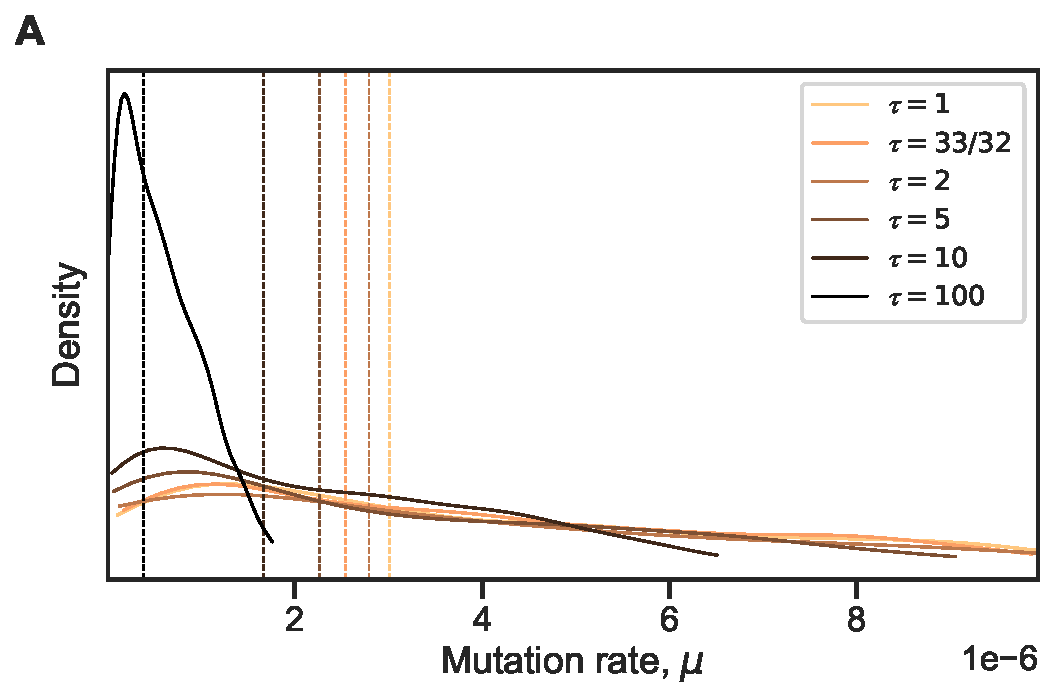
\includegraphics[width=\textwidth]{../figures/tau-A.pdf}      
  \end{subfigure}
  \begin{subfigure}{0.45\textwidth}
      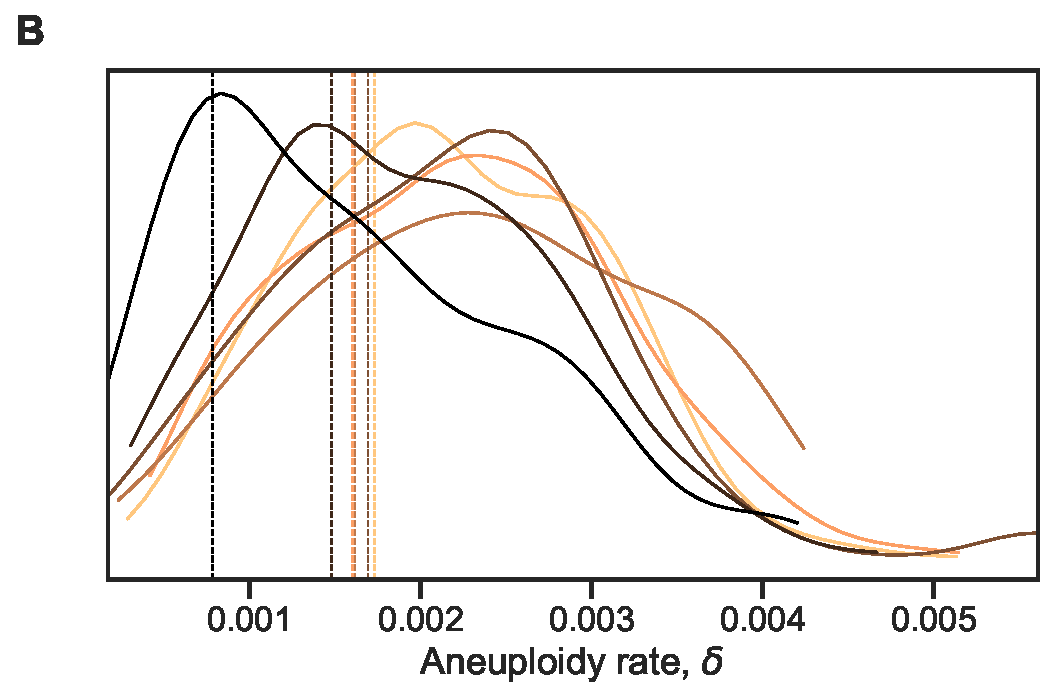
\includegraphics[width=\textwidth]{../figures/tau-B.pdf}      
  \end{subfigure}
  \\
   \begin{subfigure}{0.325\textwidth}
      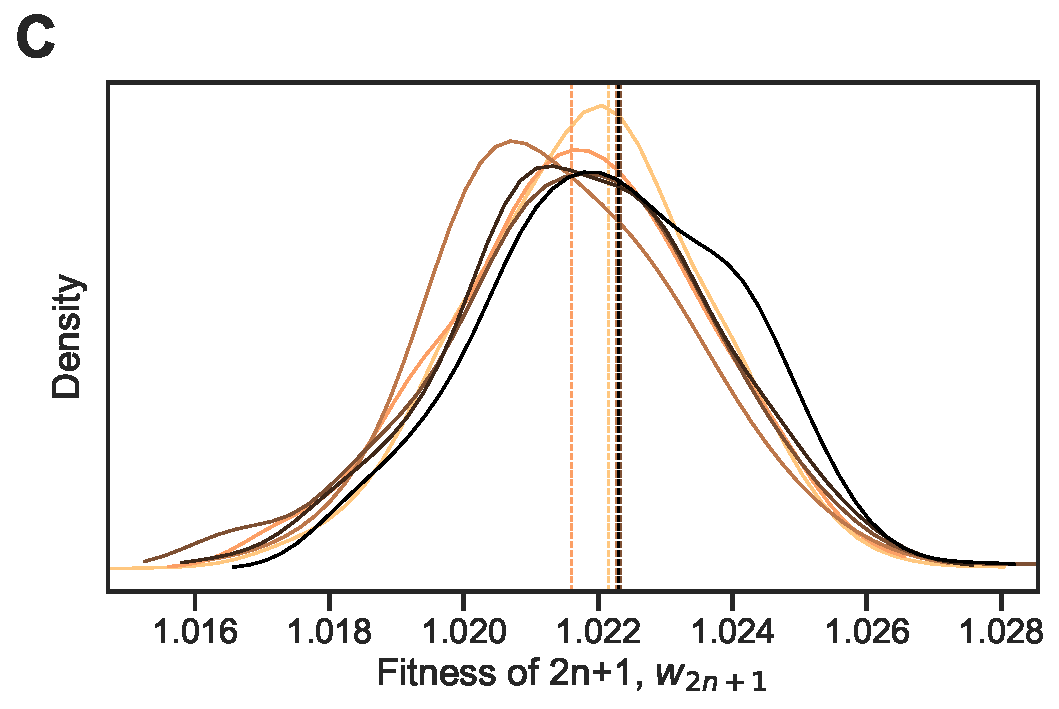
\includegraphics[width=\textwidth]{../figures/tau-C.pdf}      
  \end{subfigure}
    \begin{subfigure}{0.325\textwidth}
      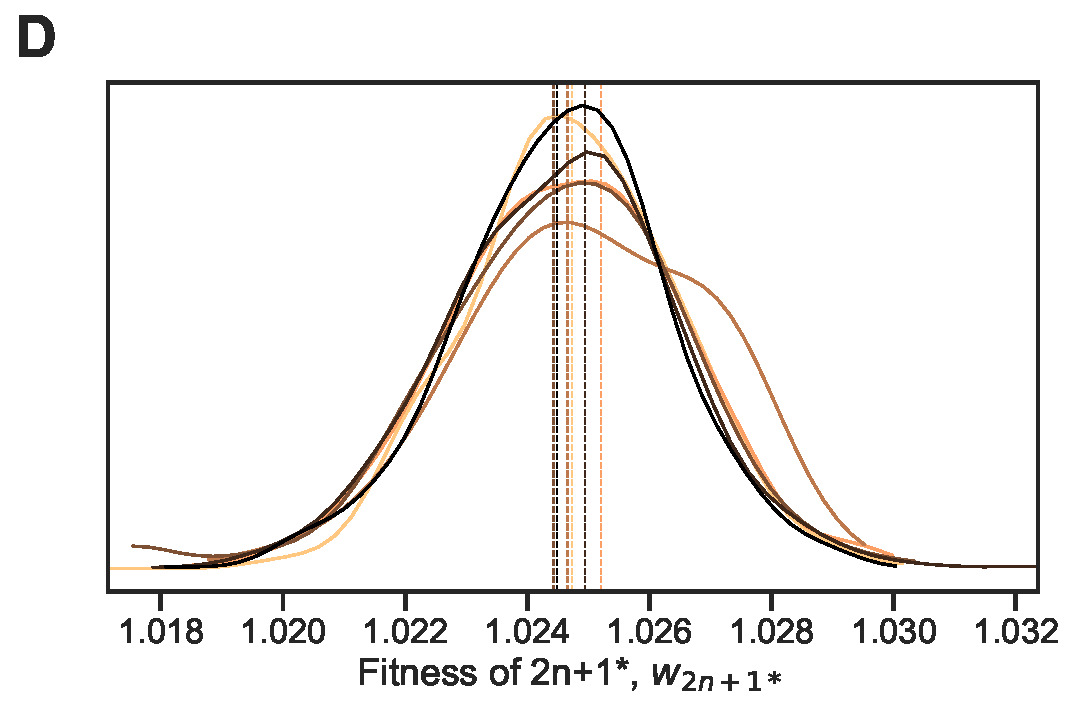
\includegraphics[width=\textwidth]{../figures/tau-D.pdf}      
  \end{subfigure}
    \begin{subfigure}{0.325\textwidth}
      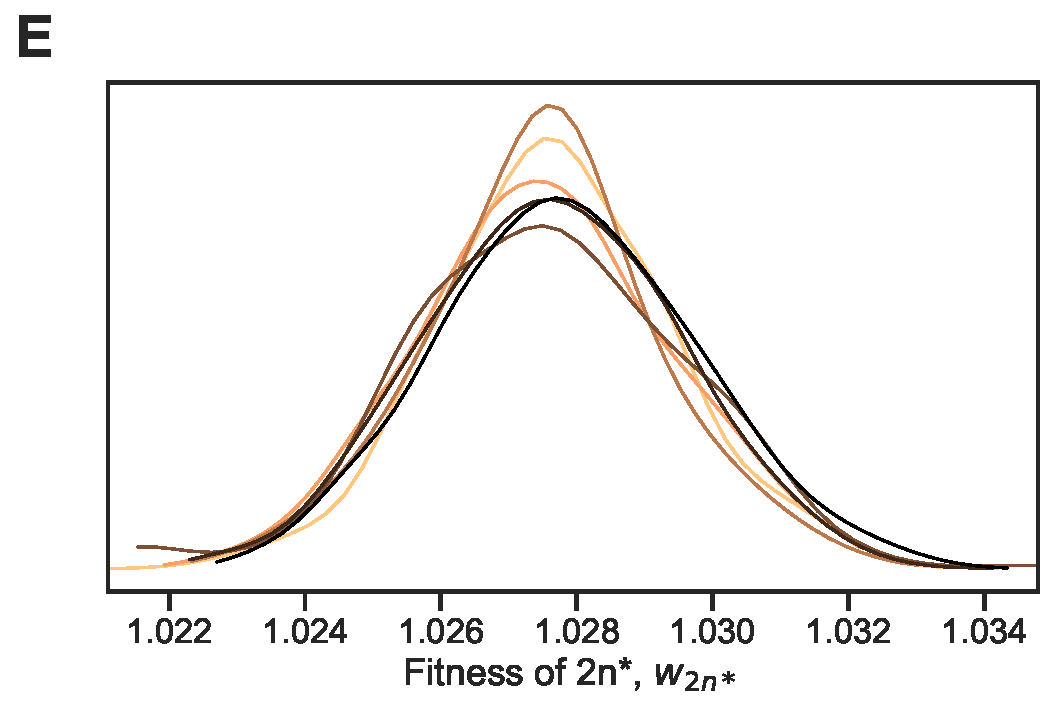
\includegraphics[width=\textwidth]{../figures/tau-E.pdf}      
  \end{subfigure}
  \\
  \begin{subfigure}{0.325\textwidth}
      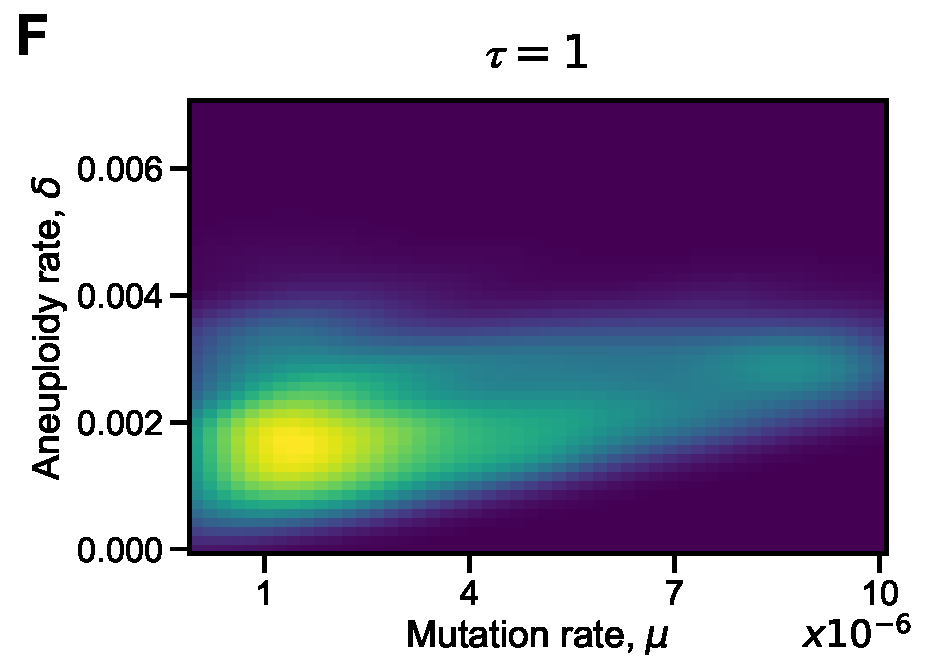
\includegraphics[width=\textwidth]{../figures/tau-joint-F.pdf}      
  \end{subfigure}
\begin{subfigure}{0.325\textwidth}
      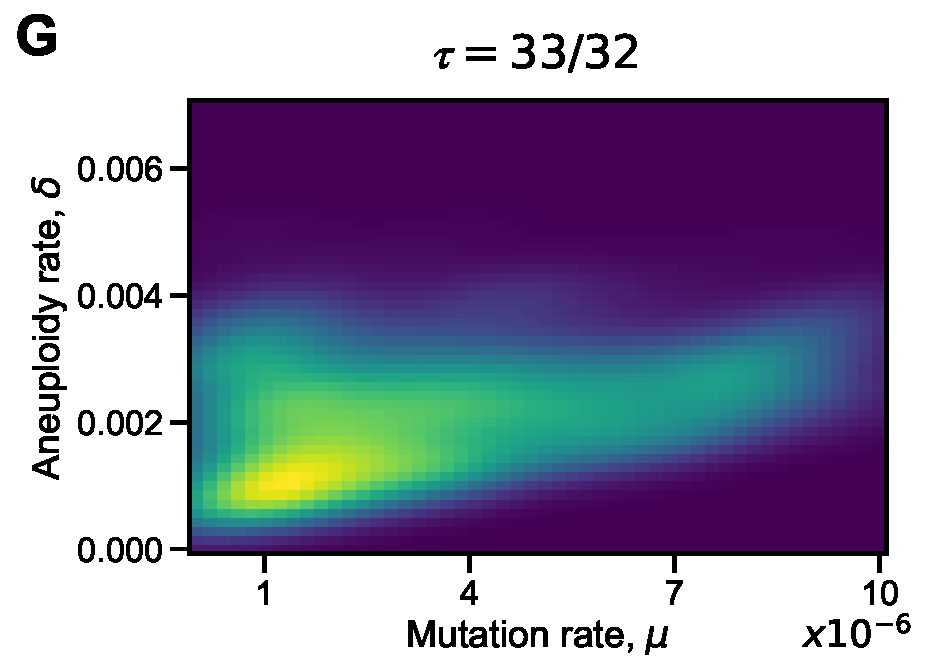
\includegraphics[width=\textwidth]{../figures/tau-joint-G.pdf}      
  \end{subfigure}
\begin{subfigure}{0.325\textwidth}
      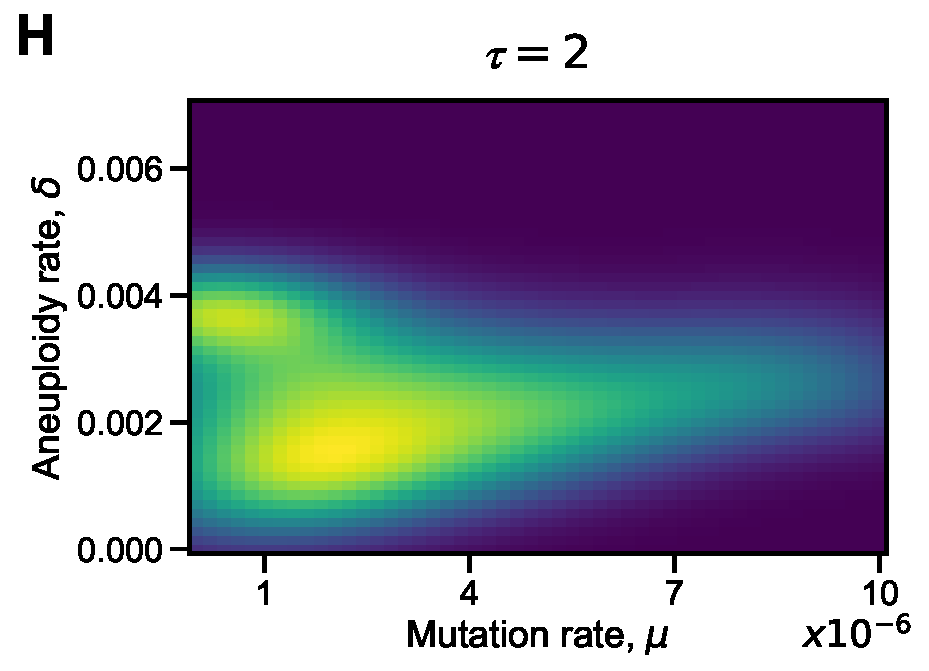
\includegraphics[width=\textwidth]{../figures/tau-joint-H.pdf}      
  \end{subfigure}
\begin{subfigure}{0.325\textwidth}
      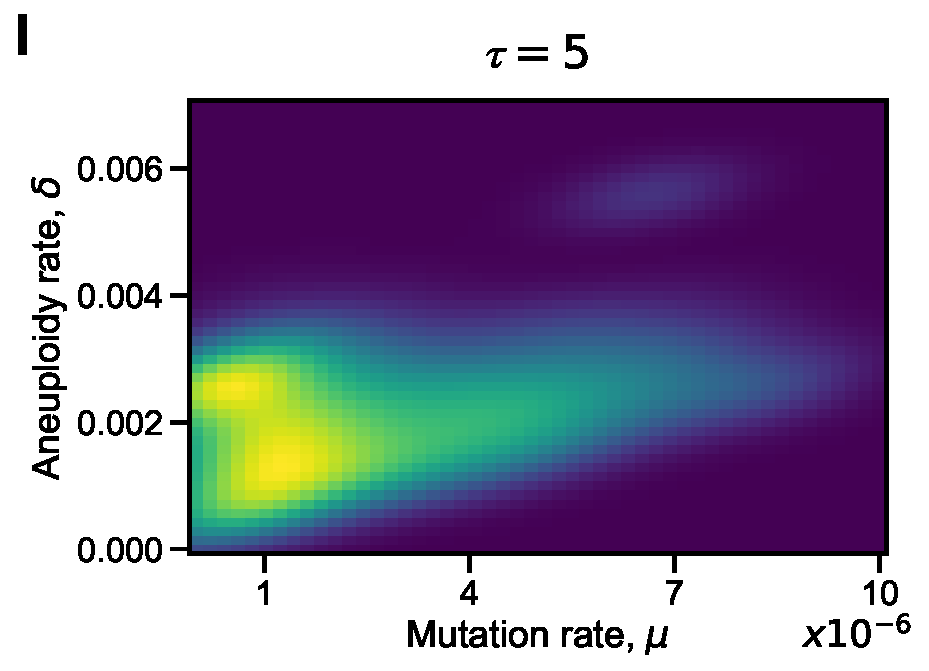
\includegraphics[width=\textwidth]{../figures/tau-joint-I.pdf}      
  \end{subfigure}
\begin{subfigure}{0.325\textwidth}
      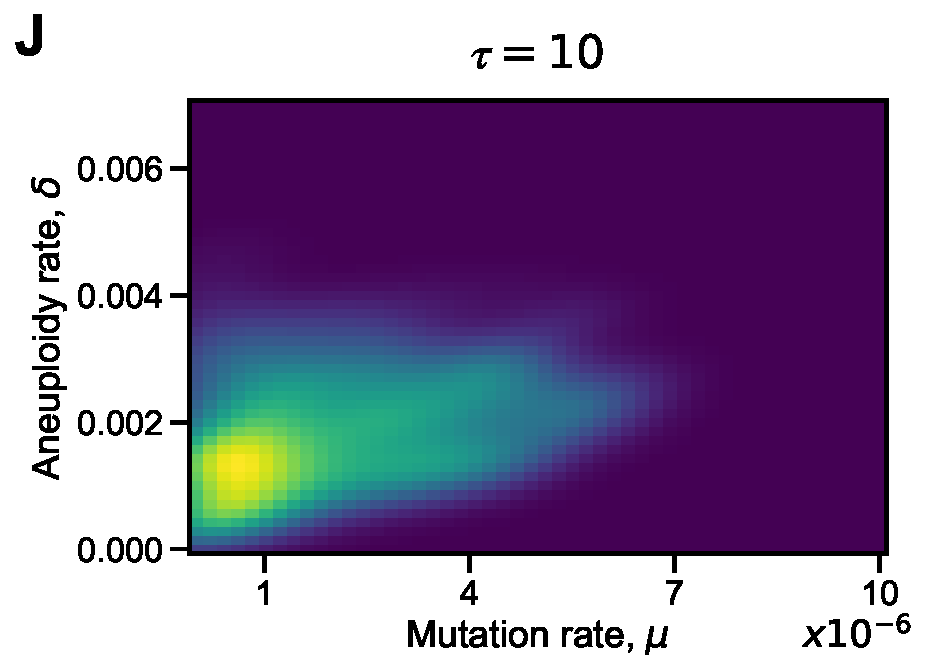
\includegraphics[width=\textwidth]{../figures/tau-joint-J.pdf}      
  \end{subfigure}
\begin{subfigure}{0.325\textwidth}
      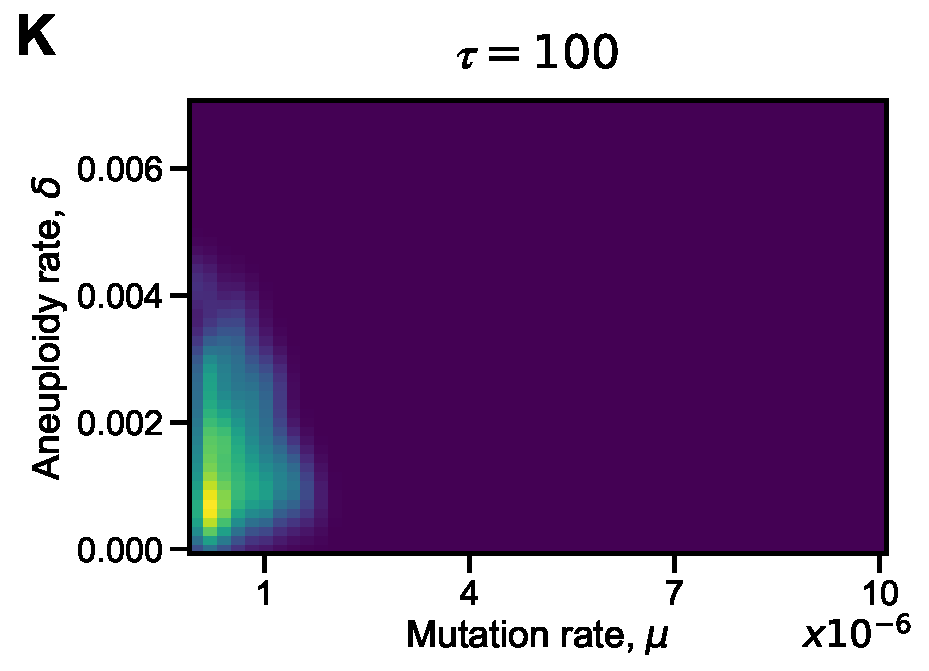
\includegraphics[width=\textwidth]{../figures/tau-joint-K.pdf}      
  \end{subfigure}
  \caption{
    \textbf{Model with elevated mutation rate in aneuploid cells.}  \textbf{(A-E)} The inferred posterior distributions for models with different values of $\tau$, the fold-increase in mutation rate in aneuploid cells (\anwt\ and \anmt). Vertical dashed lines represent the MAP (maximum a posteriori) of each distribution. When the increase in mutation rate is high, $\tau=10$ and $\tau=100$, the inferred mutation (A) and aneuploidy (B) rates tend to be lower. 
    \textbf{(F-K)} The inferred joint posterior distribution of mutation rate ($\mu$) and aneuploidy rate ($\delta$) with different $\tau$ values (dark purple and bright yellow for low and high density, respectively).
  \label{fig:tau}
  }
  \end{figure}
  
  
  
% Fig tau plots
%% generated by diff-tau-more-plots.ipynb
\begin{figure}[p]
  \centering
  \begin{subfigure}{0.75\textwidth}
      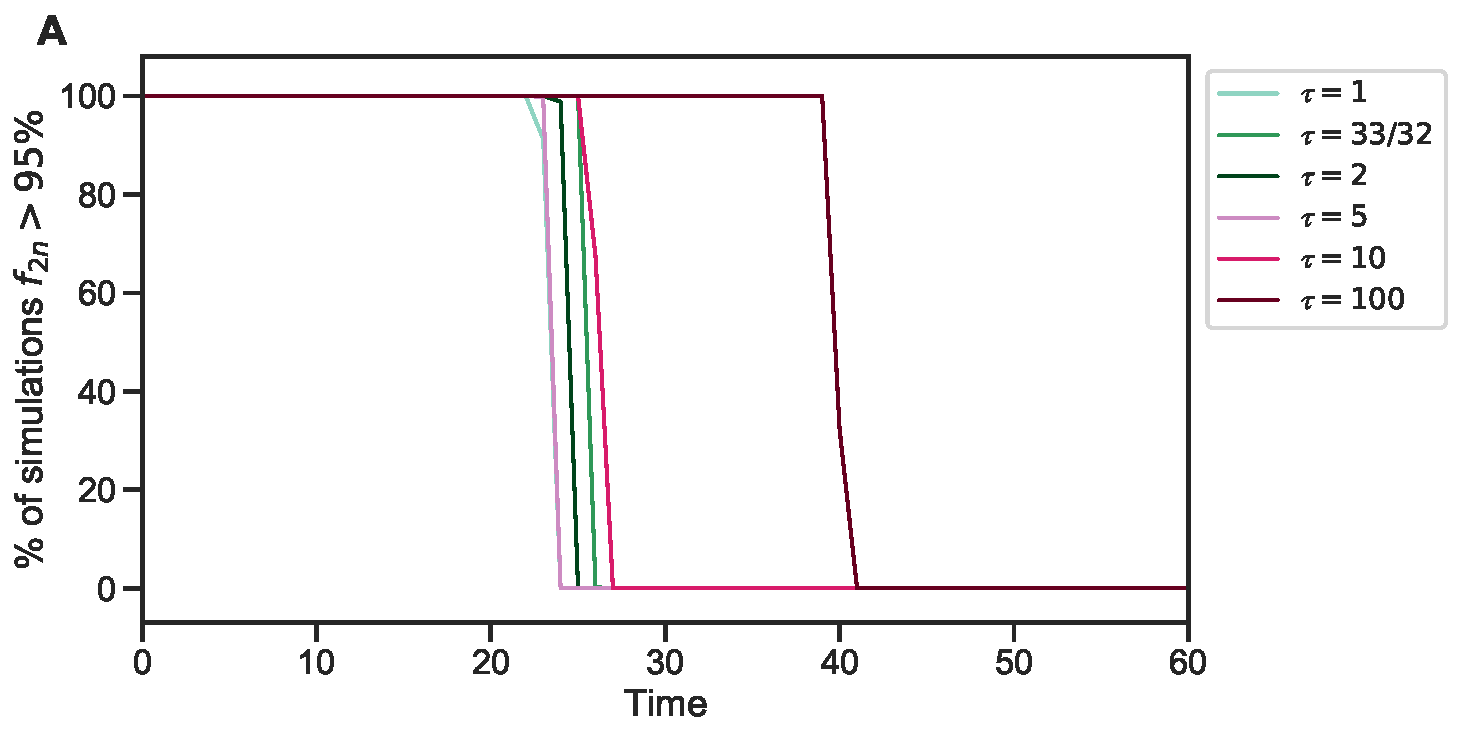
\includegraphics[width=\textwidth]{../figures/tau-diff-a.pdf}      
  \end{subfigure}
  \begin{subfigure}{0.75\textwidth}
      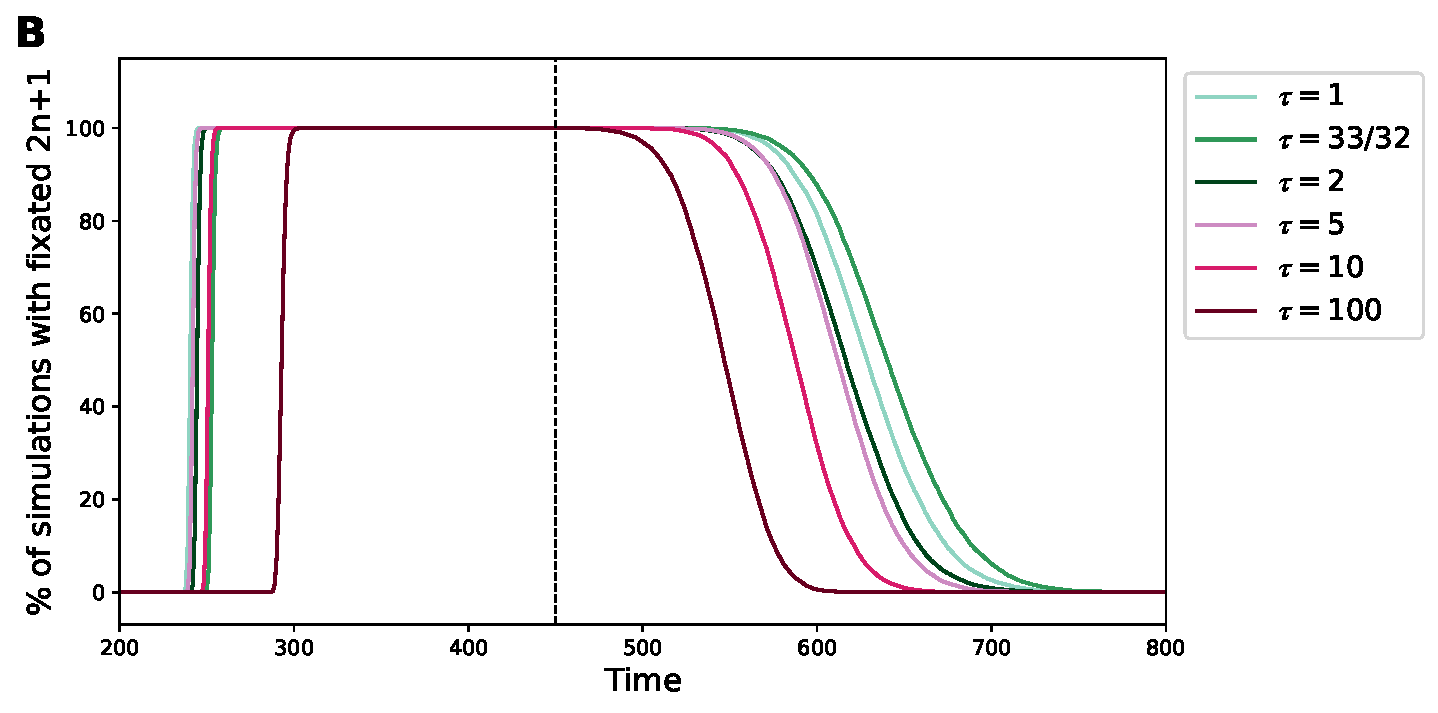
\includegraphics[width=\textwidth]{../figures/tau-diff-b.pdf}      
  \end{subfigure}
   \begin{subfigure}{0.75\textwidth}
      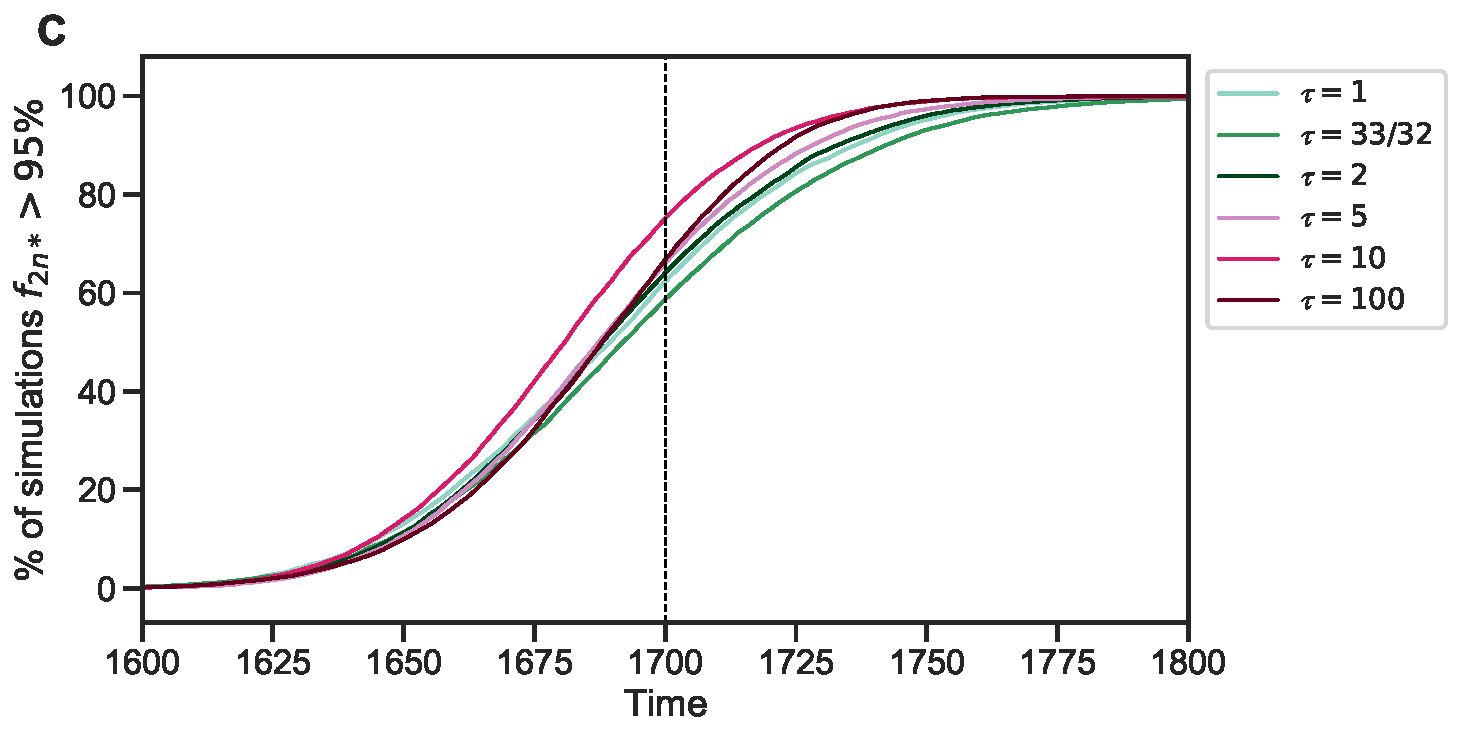
\includegraphics[width=\textwidth]{../figures/tau-diff-c.pdf}      
  \end{subfigure}
   \caption{
    \textbf{Genotype fixations for models with increased genetic instability.} We estimated the parameters for different models, each assuming a different value of $\tau$, the fold-increase in mutation rate in aneuploid cells. We then generated 10,000 simulations using the MAP estimate of each model and evaluated the fraction of simulations in which the frequency of genotype \euwt\ (\textbf{A}), \anwt\ (\textbf{B}), and \eumt\ (\textbf{C}) is above 95\% (y-axis) at each generation (x-axis). Note that \anmt\ did not fix. We can see that $\tau=100$ can be distinguished if the waiting time for $f_{\euwt}<95\%$ is known (panel~A) or if the waiting time for $f_{\anwt}>95\%$ or $f_{\anwt}<95\%$ is known (panel~B). It is harder to distinguish between $1\leq \tau \leq10$.
  }
  \label{fig:tau-plots}
\end{figure}



% Fig likelihood profile
%% generated by sensitivity-analysis.ipynb
\begin{figure}[p]
  \centering
  \begin{subfigure}{0.3\textwidth}
      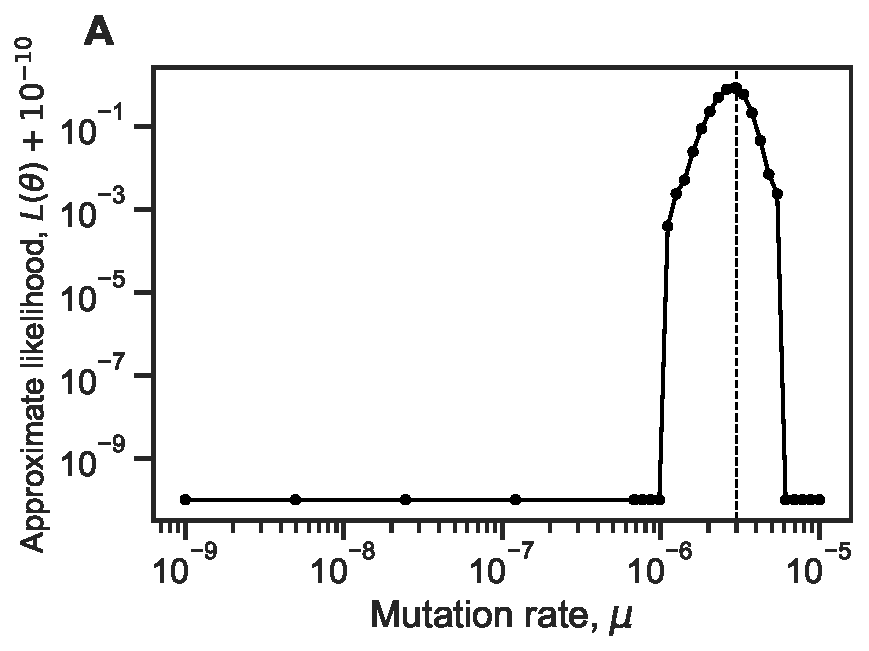
\includegraphics[width=\textwidth]{../figures/sensitivity-A.pdf}      
      \label{fig:sensitivity-mutation}
  \end{subfigure}
  \begin{subfigure}{0.3\textwidth}
      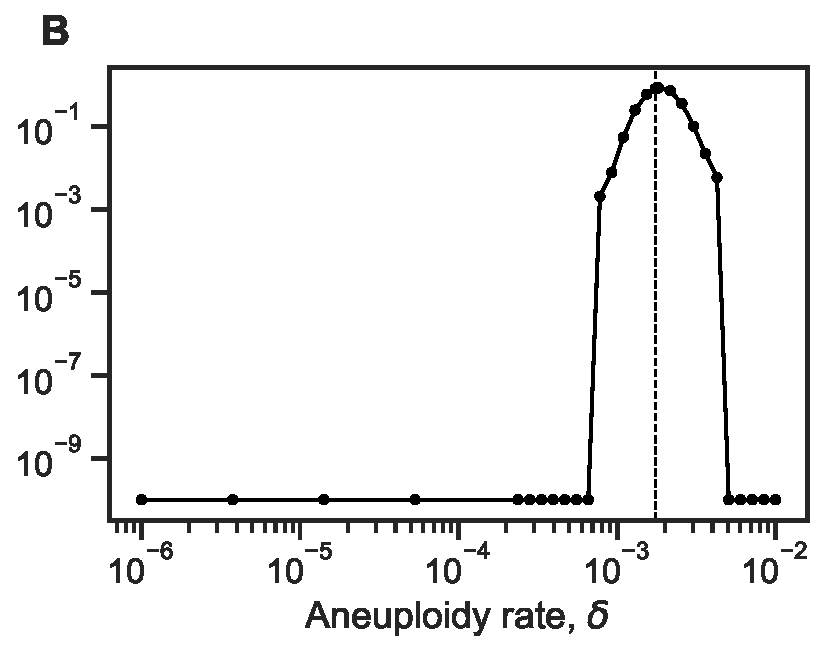
\includegraphics[width=\textwidth]{../figures/sensitivity-B.pdf}      
      \label{fig:sensitivity-aneuploidy}
  \end{subfigure}
  \\
   \begin{subfigure}{0.3\textwidth}
      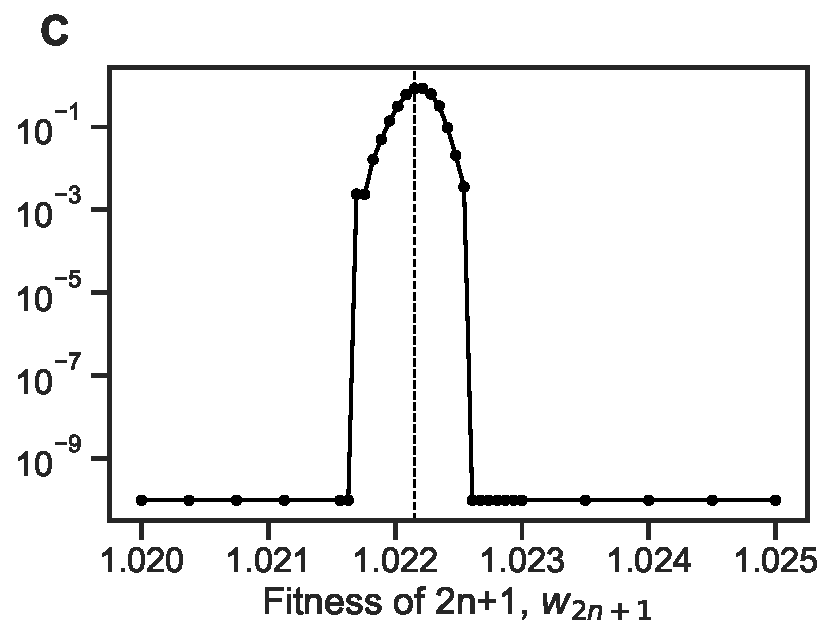
\includegraphics[width=\textwidth]{../figures/sensitivity-C.pdf}      
      \label{fig:sensitivity-anwt}
  \end{subfigure}
    \begin{subfigure}{0.3\textwidth}
      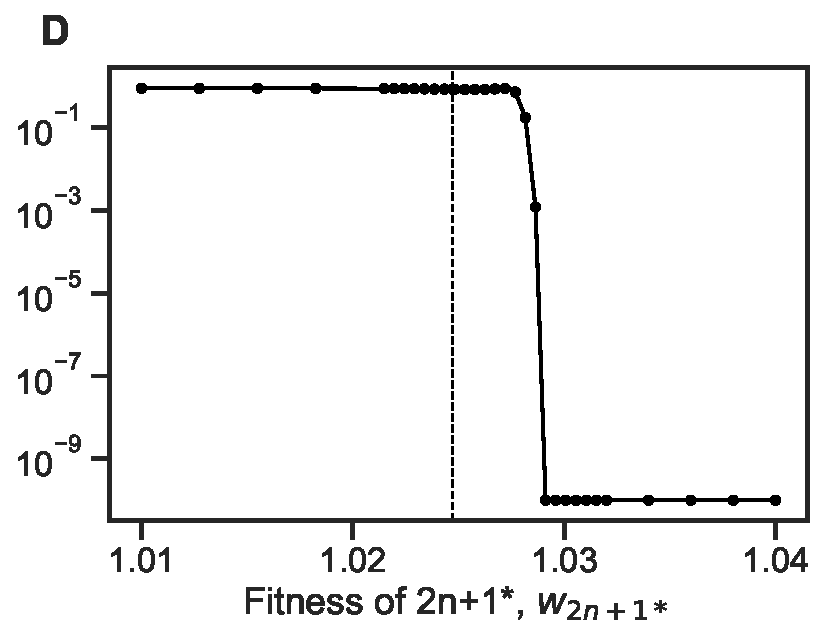
\includegraphics[width=\textwidth]{../figures/sensitivity-D.pdf}      
      \label{fig:sensitivity-anmt}
  \end{subfigure}
    \begin{subfigure}{0.3\textwidth}
      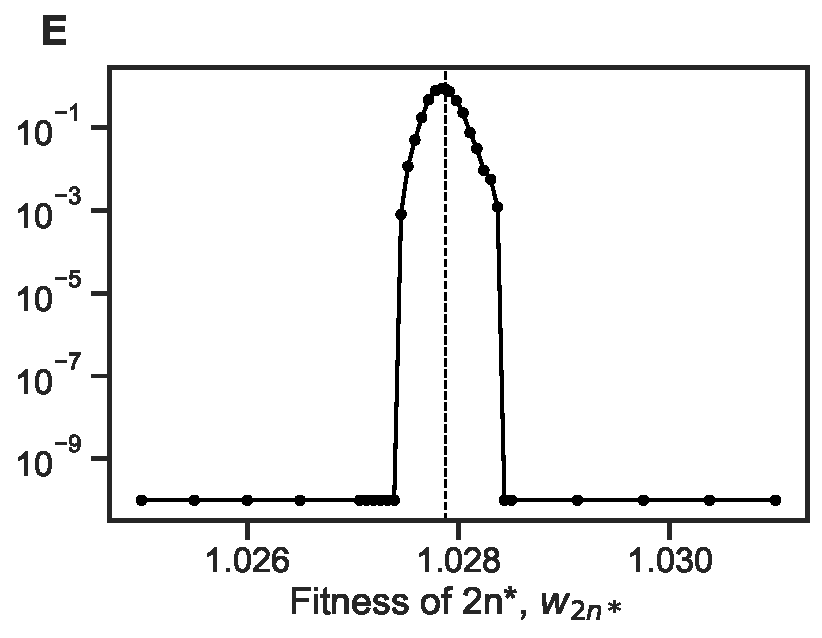
\includegraphics[width=\textwidth]{../figures/sensitivity-E.pdf}      
      \label{fig:sensitivity-eumt}
  \end{subfigure}
  \caption{
    \textbf{Likelihood profiles.} Sensitivity of the model approximate likelihood, $\likelihood(\theta)$, to changing a single parameter while the other parameters remain fixed at their MAP estimates. Dashed vertical line represents the MAP value. The prior distributions for the mutation rate and aneuploidy rate are $\mu \sim U(10^{-9}, 10^{-5})$ and $\delta \sim U(10^{-6}, 10^{-2})$, respectively. 
  }
  
  \label{fig:sensitivity}
\end{figure}


    
% Fig mu comparisons
%% generated with diff-mutation-rate.ipynb
\begin{figure}[p]
  \centering
  \begin{subfigure}{0.45\textwidth}
      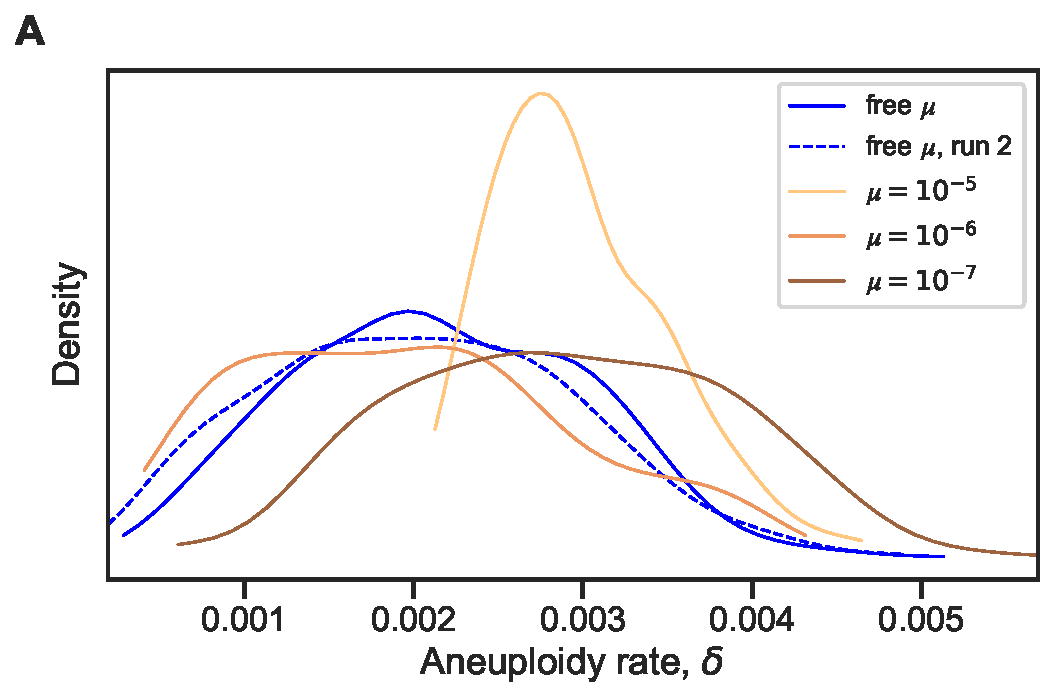
\includegraphics[width=\textwidth]{../figures/mu-A.pdf}      
  \end{subfigure}
  \begin{subfigure}{0.45\textwidth}
      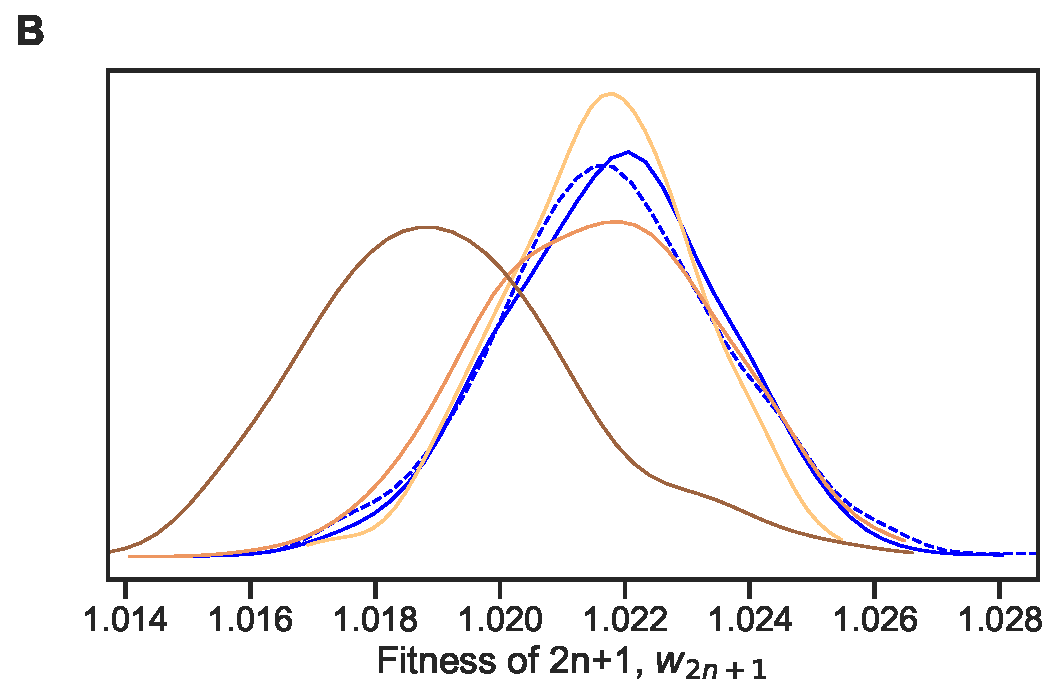
\includegraphics[width=\textwidth]{../figures/mu-B.pdf}      
  \end{subfigure}
  \\
   \begin{subfigure}{0.45\textwidth}
      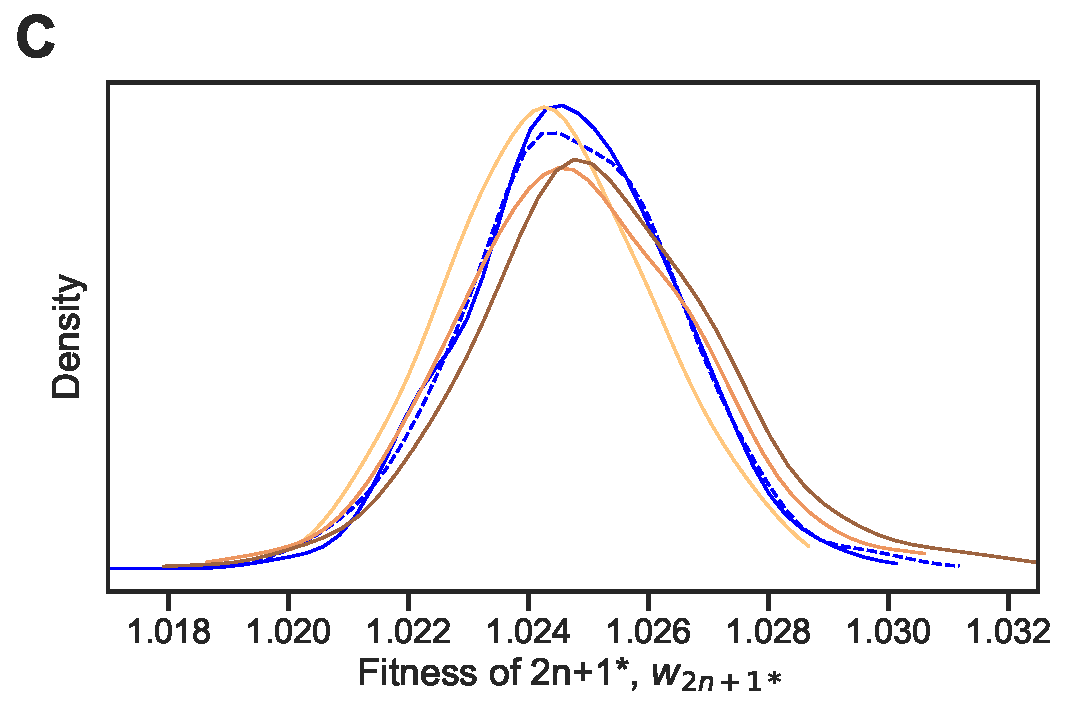
\includegraphics[width=\textwidth]{../figures/mu-C.pdf}      
  \end{subfigure}
    \begin{subfigure}{0.45\textwidth}
      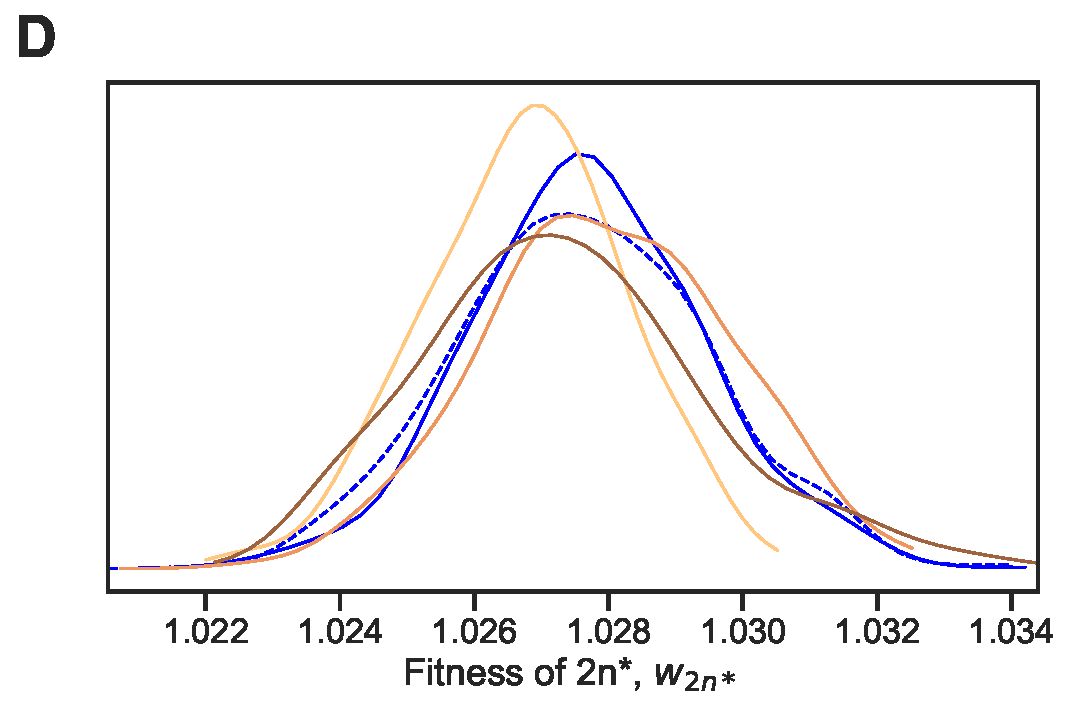
\includegraphics[width=\textwidth]{../figures/mu-D.pdf}      
    \end{subfigure}
  \caption{
    \textbf{Model with fixed mutation rate.}  \textbf{(A-D)} The inferred posterior distributions for models with free and fixed mutation rate, $\mu$. The MAP (maximum a posteriori) and 50\% HDI (highest density interval) for each model are: %MAP-and-hdi.ipynb
\textbf{free $\boldsymbol{\mu}$, run 1:}
$\delta=1.720\cdot10^{-3}\ [1.470\cdot10^{-3}-2.786\cdot10^{-3}]$, 
$w_{\anwt}=1.022\ [1.021-1.023]$,
$w_{\anmt}=1.025\ [1.024-1.026]$,
$w_{\eumt}=1.028\ [1.026-1.029]$;
\textbf{free $\boldsymbol{\mu}$, run 2:}
$\delta=2.129\cdot10^{-3}\ [1.334\cdot10^{-3}-2.695\cdot10^{-3}]$,
$w_{2n+1}=1.022\ [1.02-1.023]$,
$w_{2n+1^*}=1.025\ [1.023-1.026]$,
$w_{2n^*}=1.028\ [1.026-1.029]$;
\textbf{$\boldsymbol{\mu=10^{-5}}$:}
$\delta=2.903\cdot10^{-3}\ [2.399\cdot10^{-3}-3.156\cdot10^{-3}]$,
$w_{2n+1}=1.022\ [1.021-1.023]$,
$w_{2n+1^*}=1.024\ [1.023-1.025]$,
$w_{2n^*}=1.027\ [1.026-1.028]$;
\textbf{$\boldsymbol{\mu=10^{-6}}$:}
$\delta=1.917\cdot10^{-3}\ [9.624\cdot10^{-4}-2.447\cdot10^{-3}]$,
$w_{2n+1}=1.022\ [1.02-1.023]$,
$w_{2n+1^*}=1.025\ [1.023-1.026]$,
$w_{2n^*}=1.028\ [1.027-1.029]$;
\textbf{$\boldsymbol{\mu=10^{-7}}$:}
$\delta=2.901\cdot10^{-3}\ [2.139\cdot10^{-3}-3.671\cdot10^{-3}]$,
$w_{2n+1}=1.019\ [1.017-1.02]$,
$w_{2n+1^*}=1.025\ [1.024-1.026]$,
$w_{2n^*}=1.027\ [1.026-1.029]$.
\label{fig:mu}
  }
\end{figure}



% FIG posterior alt-prior
%% generated with alt-prior.ipynb
\begin{figure}[p]
  \centering
  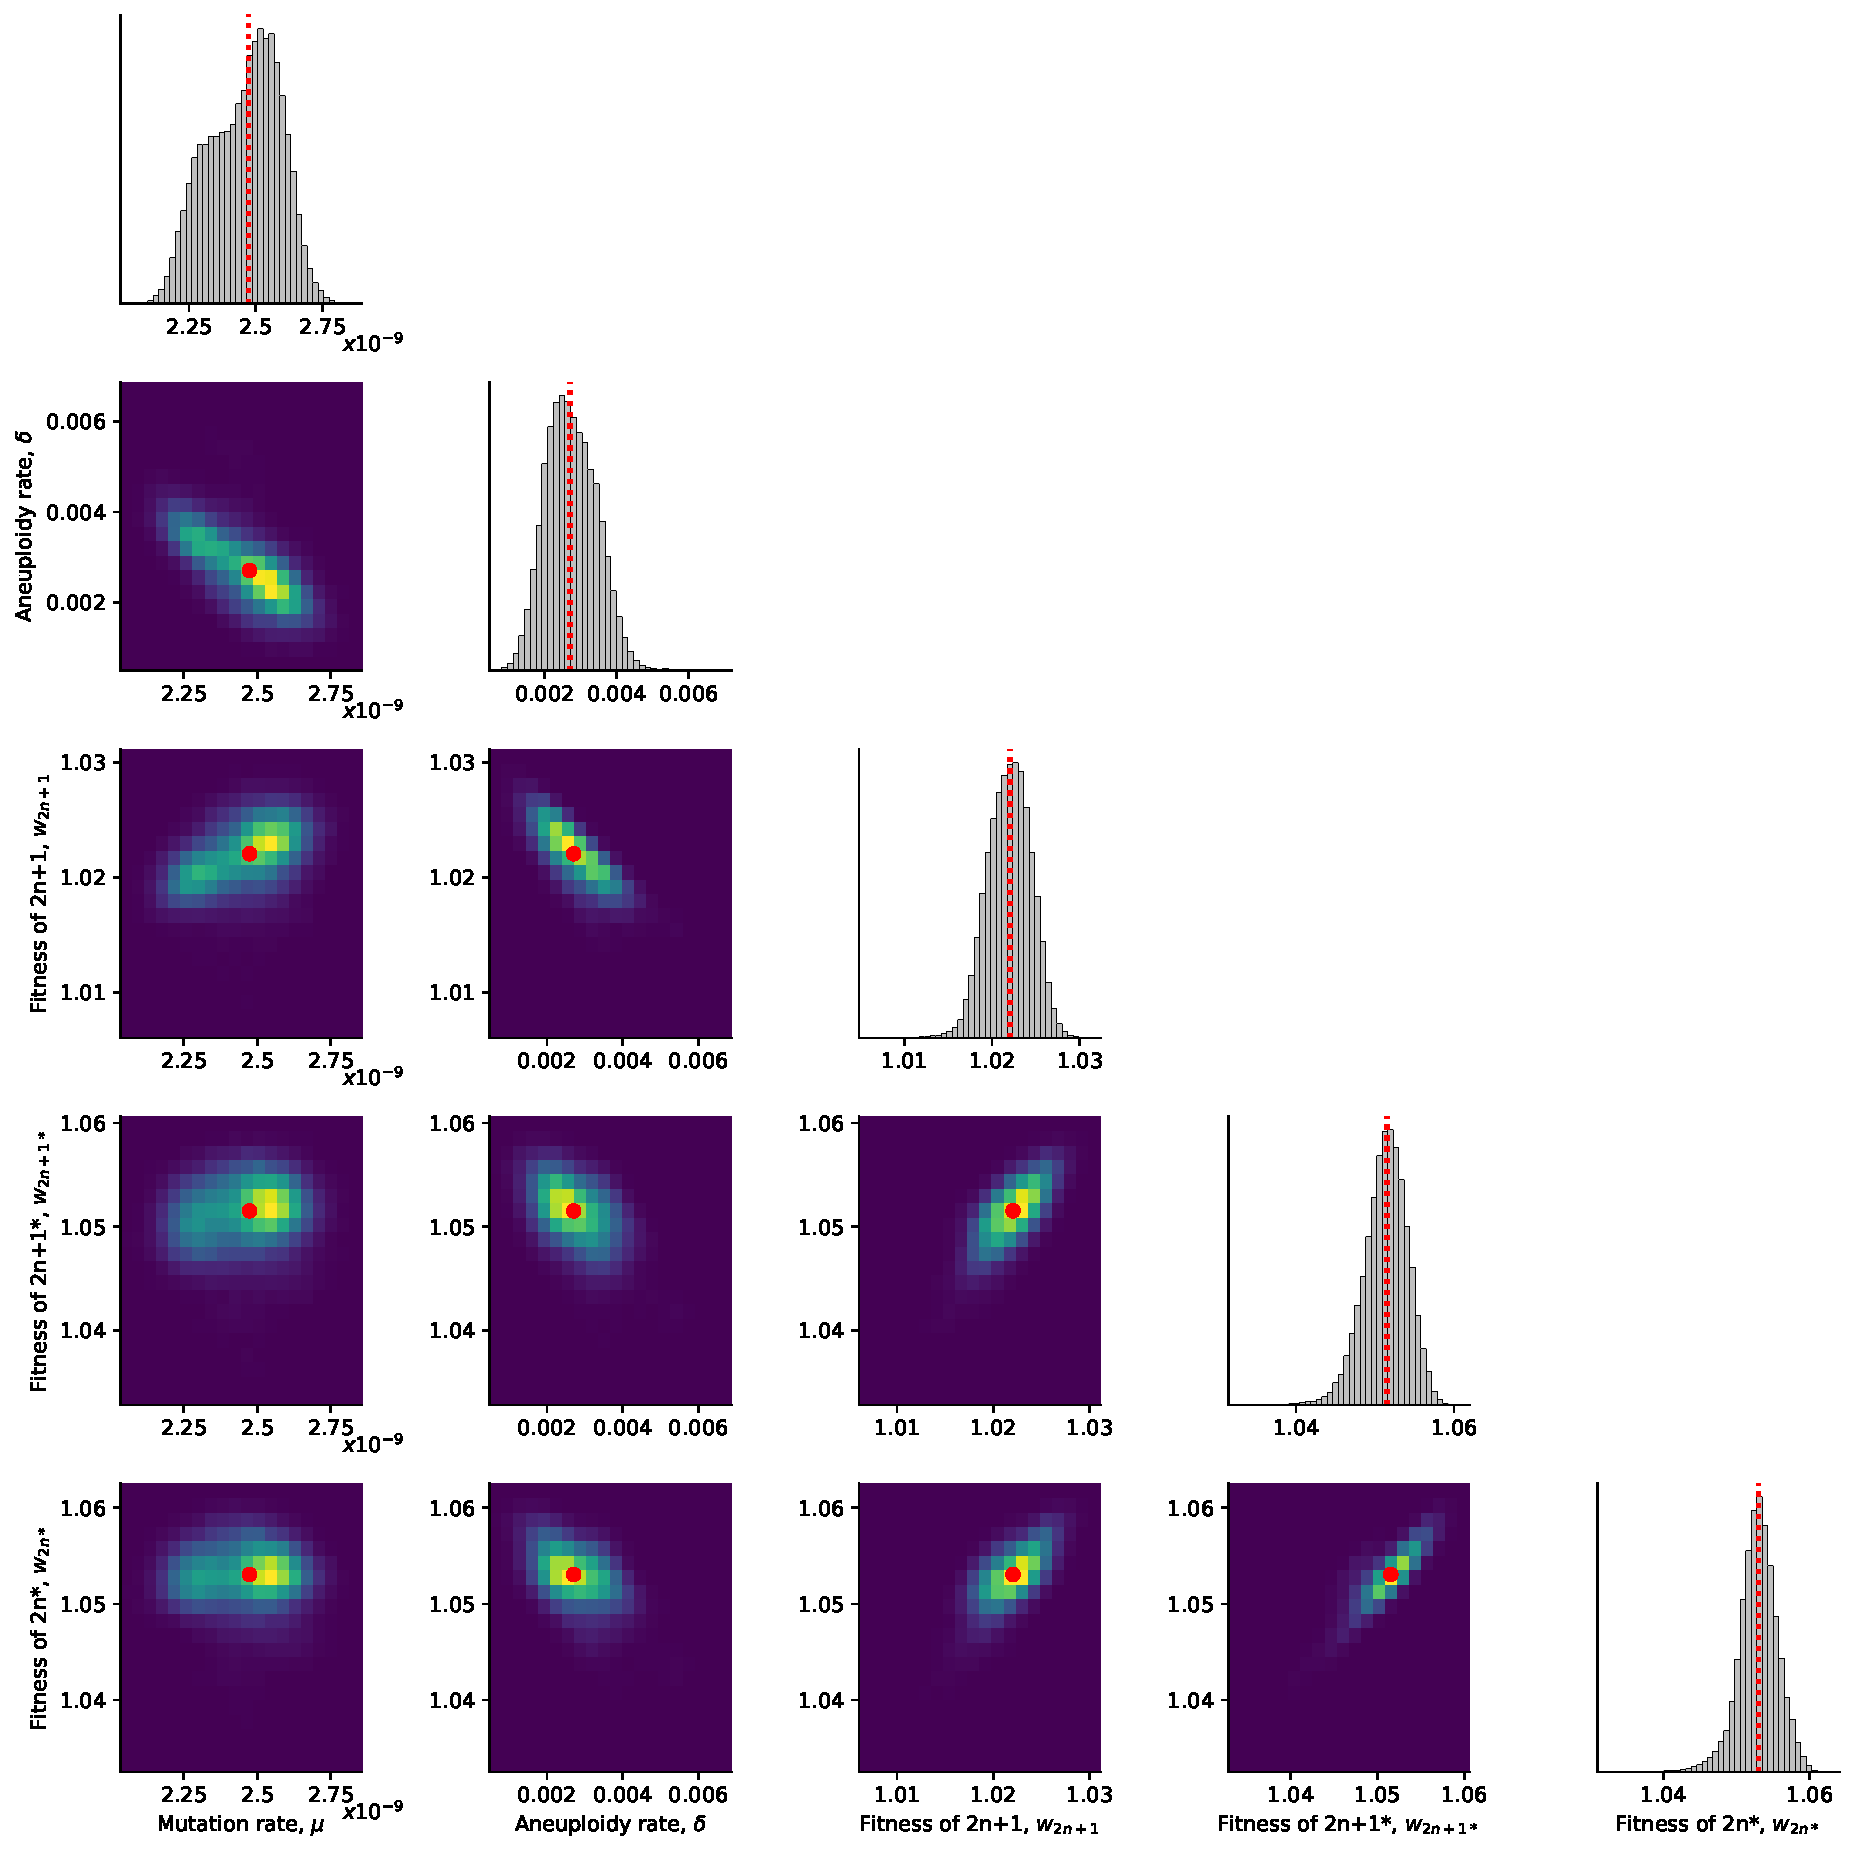
\includegraphics[width=0.9\textwidth]{../figures/posterior-alt.pdf}
  \caption{
  \textbf{Posterior distribution of parameters inferred with the extended prior distribution.}
On the diagonal, the inferred posterior distribution of each model parameter. 
Below the diagonal, the inferred joint posterior distribution of pairs of model parameters (dark purple and bright yellow for low and high density, respectively). Red markers and orange lines for the joint MAP estimate (which may differ from the marginal MAP, as the marginal distribution integrates over all other parameters).
} 
  \label{fig:posterior-alt}
\end{figure}


% FIG MAP frequency dynamics in log scale
\begin{figure}[p]
    \centering
	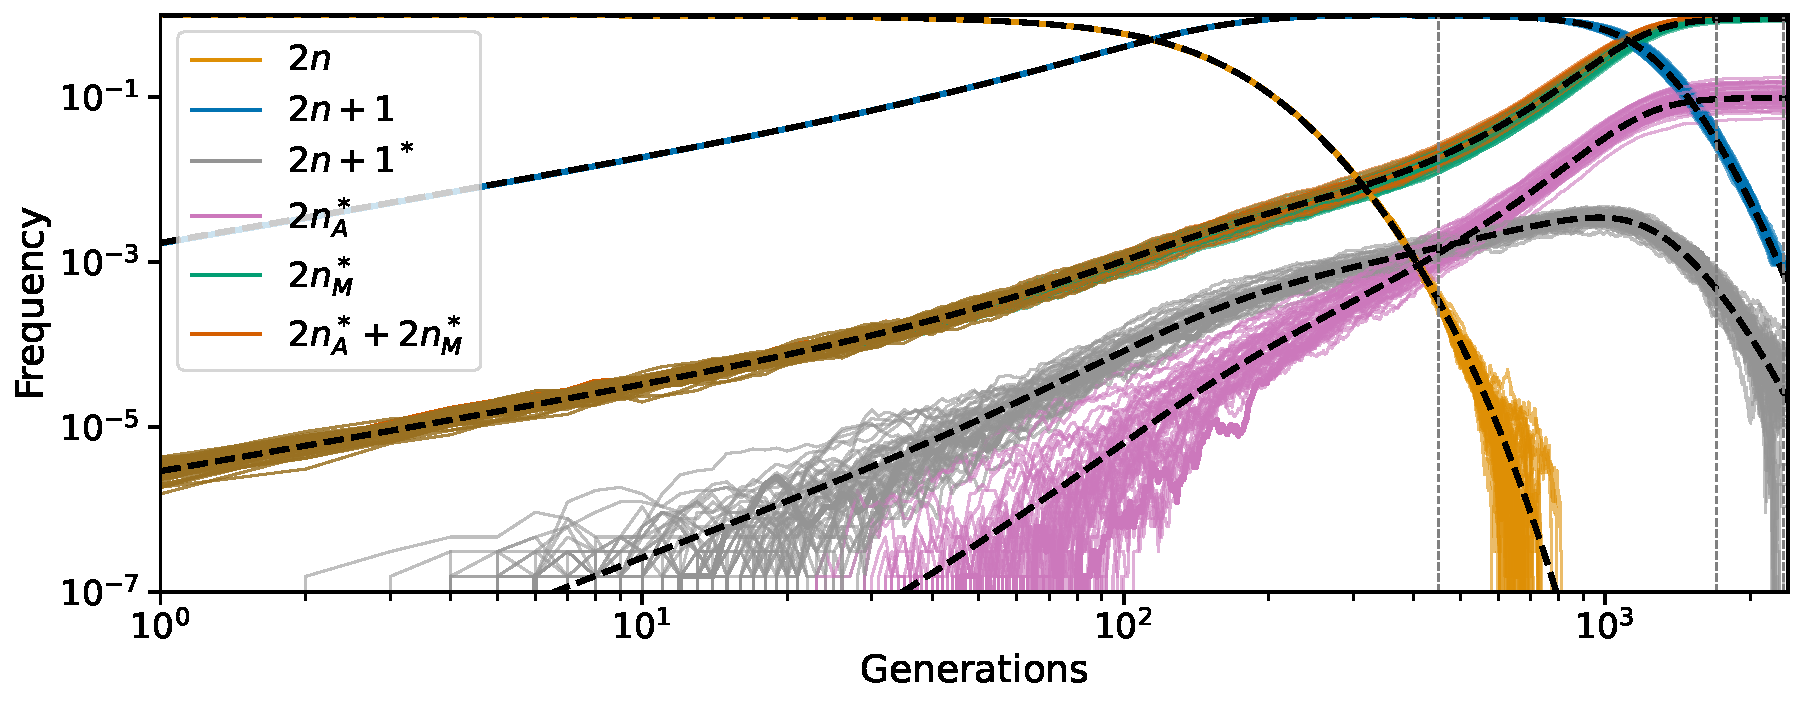
\includegraphics[width=\textwidth]{../figures/MAP_freq_dynamics.pdf}
	\caption{\textbf{Posterior predicted genotype frequencies in log-log scale.}
	Frequency dynamics of the different genotypes with MAP parameter estimates, same as \Cref{fig:FA}A, but in log-log scale. Black dashed curves for a deterministic model without genetic drift. 
	Clearly, appearance of \anwt\ and \eumtM\ is deterministic.
	Appearance of \anmt, and therefore \eumtA, is stochastic, however, the frequency dynamics are deterministic above a frequency of roughly 0.001. 
	}
    \label{fig:MAP_freq_dynamics_log}    
\end{figure}


% FIG posterior F_A supplementary
\begin{figure}[p]
	\begin{subfigure}{0.5\textwidth}
      \centering
      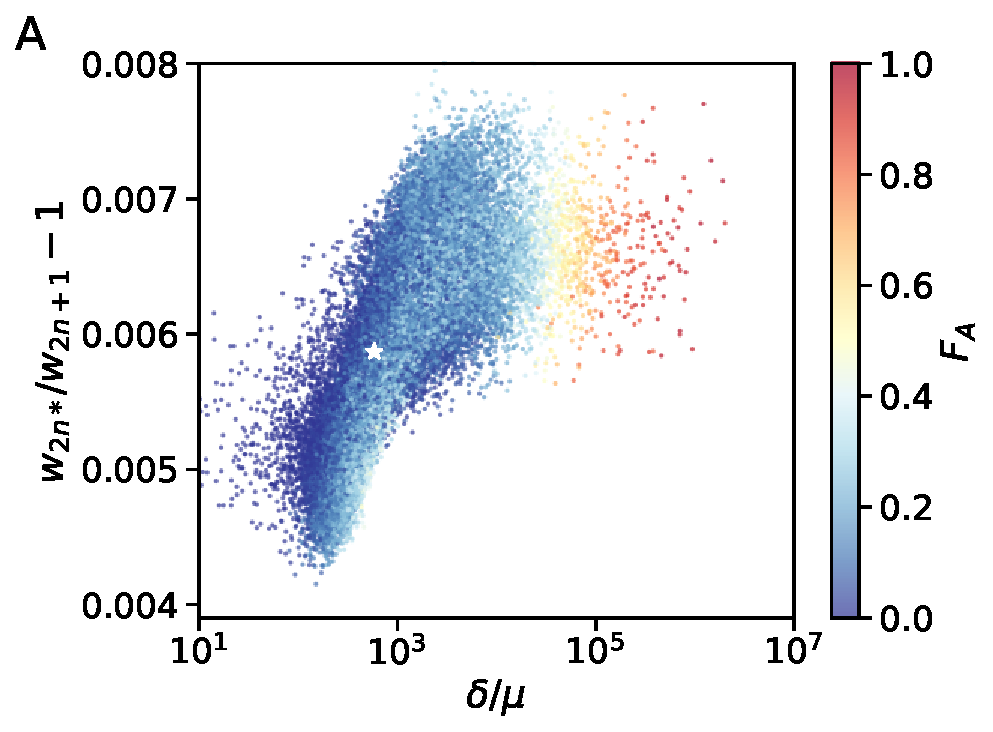
\includegraphics[width=\textwidth]{../figures/F_A_delta-mu-ratio_1.pdf}      
	\end{subfigure}
	  \begin{subfigure}{0.5\textwidth}
      \centering
      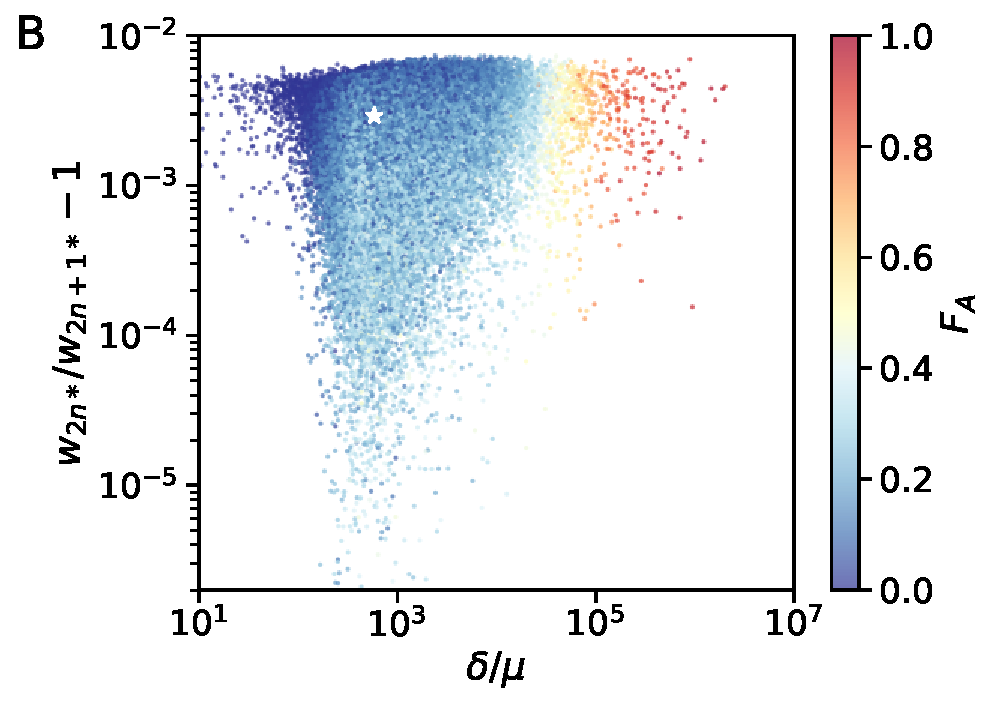
\includegraphics[width=\textwidth]{../figures/F_A_delta-mu-ratio_2.pdf}
  \end{subfigure}
	\caption{\textbf{Posterior distribution of $F_A$.}
	\textbf{(A,B)} $F_A$ values (color coded) as in \Cref{fig:FA} for different parameter choices on the x- and y-axes. White star denotes the MAP estimate.
	}
    \label{fig:posterior_FA_supp}
\end{figure}

\pagebreak

% Table - mutations
%% generated with mutation_analysis.ipynb
\begin{table}[h]
\centering
\caption{
\textbf{Mutant alleles in population $H2$.}}
\caption*{
	Mutant alleles identified in the ancestor (generation 0), aneuploid (generation 450), and evolved (generation 2,350) of population $H2$. See supplementary file.
} 
\label{table:mutations_H2}
\end{table}

% Table - mutations
%% generated with mutation_analysis.ipynb
\begin{table}[h]
\centering
\caption{
\textbf{Mutant alleles in population $H4$.}}
\caption*{
	Mutant alleles identified in the ancestor (generation 0), aneuploid (generation 450), and evolved (generation 1,700) of population $H4$. See supplementary file.
} 
\label{table:mutations_H4}
\end{table}


%% generated with WAIC.ipynb 
\begin{table}[h]
\centering
\caption{
\textbf{WAIC values for different $\tau$ values.}}
\pgfplotstabletypeset[
    col sep=semicolon,
    string type,
    every head row/.style={before row=\hline,after row=\hline},
    every last row/.style={after row=\hline},
    ]{../figures/Table_WAIC.csv} 
\caption*{
	WAIC defined in \cref{eq:WAIC}.
} 
\label{table:WAIC}
\end{table}



\end{document}  